\chapter{State of the Art} \label{chap:state_of_the_art}

In this chapter, we explore the state of the art of gesture recognition in an attempt to answer the following research questions, defined in Section~\ref{sec:introduction:research:research-questions}:
\begin{itemize}
    \item [RQ1] \textit{What are the main challenges of mid-air gesture recognition?} %We investigate the main challenges faced by developers and practitioners in the development of gesture-based applications and discuss potential workarounds. -> conclusion
    \item [RQ2] \textit{What is the performance of radar sensors for mid-air gesture recognition?}
    \item [RQ3] \textit{What types of gesture-based applications would benefit from radar sensors?} %We take a look at existing radar-based gestural interfaces in the literature. -> conclusion
    \item [RQ5] \textit{How can tools and methods aid in designing gesture-based applications that operate independently of gesture recognition logic?}
\end{itemize}
\fig~\ref{fig:state_of_the_art:graphical-summary} highlights the main contributions of this chapter and how it fits into this thesis. The rest of the chapter is divided into four main parts.
Section~\ref{sec:state_of_the_art:overview} first provides an overview of gesture based-interaction. %, to address RQ1 and RQ5.
Section~\ref{sec:state_of_the_art:lmc} then takes a look at a relatively mature vision-based technology for hand gesture interaction, called the Leap Motion Controller (LMC), to contextualize the state of the research on radar-based gesture interaction, which is explored in Section~\ref{sec:state_of_the_art:radar}.
Finally, Section~\ref{sec:state_of_the_art:this_work} positions this work within the literature.

\begin{figure}
    \centering
    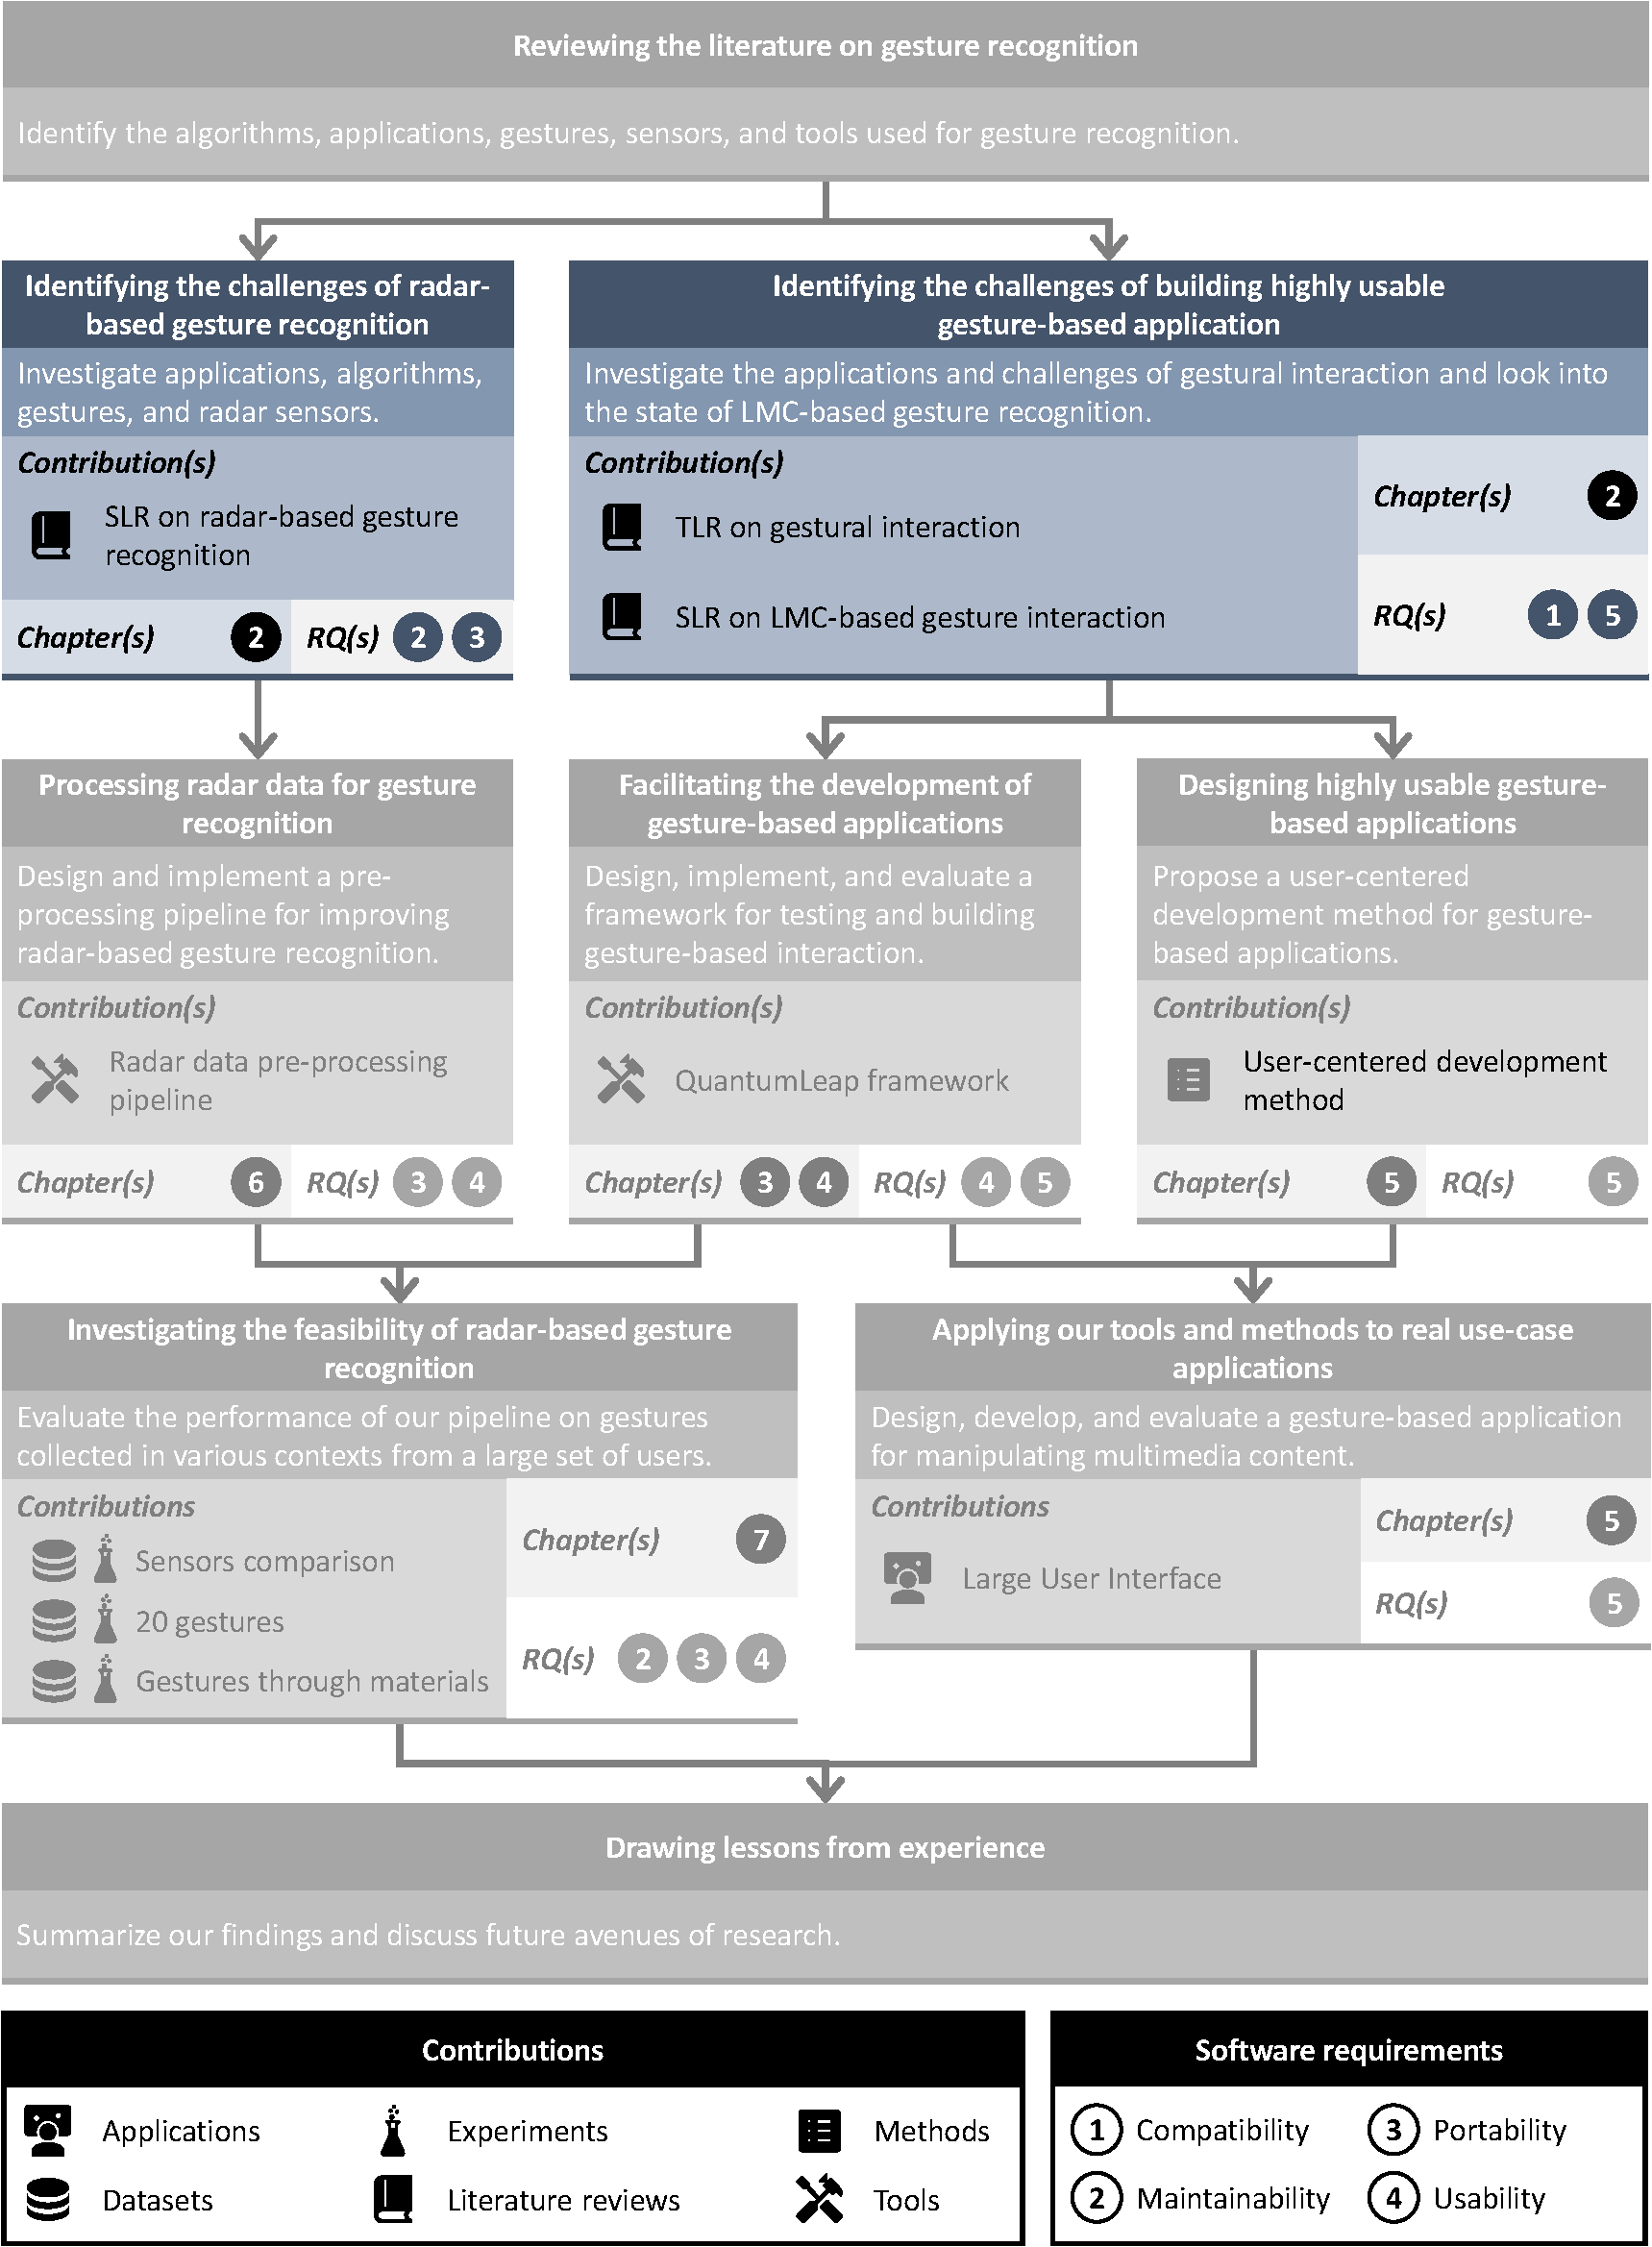
\includegraphics[width=\linewidth]{Figures/StateOfTheArt/graphical-summary-state-of-the-art.pdf}
    \vspace{-18pt}
    \caption{Main contributions of this chapter.}
    \label{fig:state_of_the_art:graphical-summary}
\end{figure}

\paragraph{Publications.} This chapter is based on three papers published in the EICS 2022 conference proceedings~\cite{Sluyters:2022:EICS}, Taylor and Francis IJHCI journal~\cite{Sluyters:2022:LUI} and ACM TiiS journal~\cite{Sluyters:2023}.

\paragraph{Resources.} The list of references from the two SLRs conducted in this chapter is available in an OSF repository at \url{https://osf.io/q43j8/?view_only=20b39a8a3d994ae4bd9ce52bfa2ded28}.

\newpage

%================================================================================%
\section{Overview of Gesture-based Interaction} \label{sec:state_of_the_art:overview}
We conducted a Targeted Literature Review (TLR) to provide a summary of the literature on the topic of gesture-based interaction. TLRs are non-systematic, in-depth, and informative reviews of the literature that keep only the references maximizing rigorousness and relevance while minimizing selection bias~\cite{Kysh:2013}.
%
Section~\ref{sec:state_of_the_art:overview:ges} first looks into gesture elicitation studies (GES)~\cite{Wobbrock:2009}, which are a great way to involve end users in the development process of gesture-based applications. 
Section~\ref{sec:state_of_the_art:overview:challenges} then discusses the main challenges faced when building gesture interaction and Section~\ref{sec:state_of_the_art:overview:applications} provides examples of gesture-based interfaces in the literature.
Finally, Section~\ref{sec:state_of_the_art:overview:summary} summarizes our findings.

%--------------------------------------------------------------------------------%
\subsection{Gesture Elicitation} \label{sec:state_of_the_art:overview:ges}
Involving end users in the development process of gesture-based applications, \eg by conducting a GES to identify a set of highly-guessable gestures, is crucial to provide a good user experience.
GESs were presented by Wobbrock \etal~\cite{Wobbrock:2009} as a participatory design method for understanding, collecting, exploring, and analyzing users preferences for gestures suitable to a particular context of use~\cite{Calvary:2003}, which is made up of a user, a device or computing platform, an environment, and some related tasks. The GES outcome consists of a characterization of users' gesture input behavior in terms of user-defined gestures~\cite{Grijincu:2014} with valuable information for designers, practitioners, and end users regarding the consensus levels between participants, computed as agreement or co-agreement scores~\cite{Vatavu:2014b}, or more recently agreement rates~\cite{Vatavu:2015}.
Vatavu and Zaiti~\cite{Vatavu:2014b} suggested that a correlation exists between the agreement rate and the recall rate, \ie a higher agreement usually means that participants recall their gesture propositions better.
This method has been widely applied to a large array of individual contexts of use (see~\cite{Villarreal:2020} for a systematic literature review), such as in Augmented Reality~\cite{Piumsomboon:2013}, smartphones~\cite{Ruiz:2011}, TVs~\cite{Vatavu:2014b,Morris:2012,Dong:2015}, and holograms~\cite{Pham:2018}.

The vast majority of these GESs target a single context of use, \ie a single category of users issuing gestures with a dedicated device in a given environment, thus posing the question of their transferability and applicability to other contexts. 
%
Among the few GESs targeting multiple contexts of use, Anthony \etal~\cite{Anthony:2013} observed that stroke gestures issued by a stylus \vs finger were inconsistent. In a systematic literature review of mid-air gestures, Groenewald \etal~\cite{Groenewald:2016} observed that gesture sets were largely inconsistent with each other and that no holistic study existed to address this problem.
%
Wittorf and Jakobsen~\cite{Wittorf:2016} elicited mid-air gestures for interacting with elements on wall displays. They noted that users' hand poses were often irrelevant to the meaning of the proposed gestures (\eg a \textit{swipe} gesture can be performed with any hand pose). Instead, the meaning was conveyed through the direction or expression of the gesture. When referents resembled actions associated with touch interactions, the proposed gestures were often larger-scale versions of common touch gestures. Users tended to favor gestures resembling the physical manipulation of objects. Overall, compared to other studies on smaller displays, the participants of this study proposed larger and more physically-based gestures.
%
Similarly, Ortega \etal~\cite{Ortega:2017} conducted a GES for eliciting multi-touch and mid-air gestures for 3D navigation in a procedurally generated universe. They found significant overlap between the proposed touch and mid-air gestures, and observed that most participants found mid-air gestures more immersive and intuitive than touch gestures.

Cross-context consistency has been initially addressed in three studies. Dingler \etal~\cite{Dingler:2018} designed a gesture set for reading via RSVP (Rapid Serial Visual Presentation) that ensures consistency across three devices, \ie a smartwatch, a smartphone, and smart glasses. A first GES collected gesture proposals for all three device types at once and considered the gesture proposals for all devices when constructing the final gesture set. They defined two new measures: the \textit{transferability score} (\ie how well a set of commands learned on one device can be ported to another) and the \textit{consistency score} (\ie the mean of all transferability scores between all devices). A second experiment with 18 participants validated the transferability of their gesture sets across devices. More recently, Vogiatzidakis and Koutsabasis~\cite{Vogiatzidakis:2019} computed a consistency rate $CR(C)$ by computing the agreement for one user performing one of 14 commands on seven home devices (\ie a smart television, speakers, video player, audio player, air conditioner, lights, and blinds). For this purpose, they computed the agreement rate for a single command and a single user, but for different devices. 
In the same home context of use~\cite{Vogiatzidakis:2020}, they introduced a consistency routine process that checks gesture proposals for consistency before incorporating them into a real system.

% In conclusion, apart from the three last studies, we are not aware of any work investigating gesture consistency, either in general or for mid-air interaction,  across different types of media objects. Some papers study users' preferred gestures either for a particular media type or for a well-defined set of actions, but independently of media types or without considering inter-media consistency. When consistency is addressed, it is across different device types, but not across different media types, which all have their generic and specific sets of functions. While recent work reported that gestures elicited on different devices are not consistent, previous work did not investigate how to ensure consistency across media types.


%--------------------------------------------------------------------------------%
\subsection{Challenges} \label{sec:state_of_the_art:overview:challenges}
This section highlights the main challenges that developers and practitioners may face in the development of gesture-based applications and discusses potential workarounds.


\subsubsection{Sensor Limitations} \label{sec:state_of_the_art:overview:challenges:sensors-limitations}
Depending on their technology, sensors may be subject to a series of limitations. For example, vision-based sensors such as the LMC are sensitive to environmental conditions~\cite{Yeo:2017}, limited field of view~\cite{Hayashi:2021}, occlusion~\cite{Brandon:2014}, and may raise privacy concerns~\cite{Avrahami:2018}. On the other hand, radar-based systems preserve privacy and can function in darkness, but are sensitive to clutter, noise, and interference. Some wearable sensors (\eg smart rings, watches, data gloves) may provide more accurate data, but this higher accuracy comes at the cost of practicality. Besides the limitations intrinsic to their technology, most sensors result in a compromise between a series of factors, including cost, field of view, framerate, and resolution.

Practitioners should consider these limitations into account in the design of their gesture-based user interfaces. Gesture sets should be designed such that the sensor(s) can differentiate between each gesture and the selected sensor(s) should suit the context of use of the UI. 
%
When no single sensor adequately fulfills the requirements of an application, integrating multiple sensors through sensor fusion should be considered to combine their strengths and enhance overall system performance. 
%
For instance, Marin \etal~\cite{Marin:2014} fed features extracted from two vision-based sensors, an LMC and a Microsoft Kinect, into a Support Vector Machine (SVM) classifier to improve gesture recognition accuracy. 
%
Kalman filters are a powerful tool for sensor fusion, thanks to their ability to estimate the state of a system (\eg the position of individual hand joints) in real time from a series of noisy measurements from one or more sensors. They can help improve the reliability of gesture recognition in challenging conditions, like occlusion or varying lighting conditions.
%
For example, Ovur \etal~\cite{Ovur:2021} used Kalman filters to merge data from two LMCs positioned at different angles. This approach enabled reliable hand pose tracking, even when one part of the hand obscured another from the viewpoint of one sensor (\ie self-occlusion).
%
Similarly, Ponraj and Ren~\cite{Ponraj:2018} leveraged Kalman filters to combine LMC data with two flex sensors integrated into a glove. The addition of flex sensors enabled more accurate hand pose recognition, particularly when parts of the hand were not visible to the LMC.


\subsubsection{Jitter} \label{sec:state_of_the_art:overview:challenges:jitter}
\label{sec:noise}
Jitter can be caused by tracking errors, sensor noise, or even a slight tremor in the user's hands. Too much jitter can significantly hinder interactions with gesture-based applications~\cite{Pavlovych:2009}, as it may induce recognition errors, as well as a lack of precision when pointing and selecting, especially on larger screens. It is thus important to perform at least some filtering in a gesture recognition pipeline to increase the precision of pointing and provide cleaner data to the gesture recognizers.

Depending on the sensors and recognition algorithms used, some filtering may already occur at several points in the pipeline. For instance, the LMC applies some filtering on the data that it provides~\cite{Colgan:2017}, and the sampling performed by some recognizers such as 3 cent~\cite{Caputo:2017}, Jackknife~\cite{Taranta:2017}, or \$P+~\cite{Vatavu:2017a} can act as a low pass filter. However, additional filtering may be applied to further smoothen the data.

Filters should be carefully selected and configured to provide reasonable smoothing while keeping latency low~\cite{Pavlovych:2009} and minimizing the risk of introducing inaccuracies. In \cite{Casiez:2012}, Casiez \etal propose the 1€ filter, a simple and fast filter based on double exponential smoothing that promises good smoothing and low latency for both fast and slow motion. They compare it to other filtering methods, namely, moving average, single and double exponential~\cite{LaViola:2003}, and Kalman, and show that it manages \textit{state-of-the-art} performance while being faster to execute.


\subsubsection{Gesture Production Variability} \label{sec:state_of_the_art:overview:challenges:production-variability}
Some variability in gesture production is usually observed both in gestures performed by a single user (intra-user variability) and by several users (inter-user variability). This variability can originate from differences in execution (\eg speed, trajectory) or in anatomy (\eg hand size, posture). If ignored, it can reduce gesture recognition accuracy and thus negatively impact the usability of gesture-based applications.

Several techniques exist to deal with gesture production variability. For instance, increasing the size of the training set by including more gesture samples produced by a greater range of users often results in higher recognition accuracy~\cite{Vatavu:2013}.
However, large training sets may increase execution time and are time-consuming to create. Synthetic data generation has been shown to increase accuracy while requiring little to no effort from developers~\cite{Taranta:2016, Leiva:2015}. A series of tools, such as MAGIC~\cite{Ashbrook:2010, Kohlsdorf:2011, Kohlsdorf:2013} and Gesture à Go Go~\cite{Leiva:2015}, have been developed to quickly augment gesture datasets with synthetic gestures. In~\cite{Maghoumi:2019}, Maghoumi and LaViola used synthetic gesture generation in their DeepGRU recognizer to avoid overfitting.

To increase accuracy for single users, recognizers could be trained only on gestures performed by this specific user. Indeed, template-matching algorithms have been shown to perform better in user-dependent settings~\cite{Vatavu:2013}, \ie where the recognizers are trained and tested with samples produced by the same user. 
Coupled with synthetic data generation, one could achieve high accuracy with little input from the target user. 

Finally, gesture recognition algorithms can be designed to accommodate some gesture production variability: for example, techniques such as Dynamic Time Warping (DTW) and spatial sampling can help deal with differences in gesture articulation speed~\cite{Taranta:2017, Vatavu:2013}.


\subsubsection{Static vs. Dynamic Gestures} \label{sec:state_of_the_art:overview:challenges:static-vs-dynamic}
Two main gesture types emerge from popular taxonomies: static and dynamic gestures~\cite{Aigner:2012,Vatavu:2008,Piumsomboon:2013,Choi:2014}. Inspired by~\cite{Vatavu:2008}, we propose the following definitions: a \textit{static} gesture is a particular configuration of the body or body parts at one instant of time, whereas a \textit{dynamic} gesture corresponds to a particular motion of the body or body parts through time. 
Different techniques may be leveraged to recognize each type of gesture. For instance, static gestures can be recognized at each frame to provide real-time recognition, while dynamic gestures are usually extracted from the raw stream of data (\ie gesture segmentation) before attempting to recognize them.


\subsubsection{Gesture Segmentation} \label{sec:state_of_the_art:overview:challenges:segmentation}
One of the greatest challenges in continuous gesture recognition is gesture segmentation, \ie extracting user gestures from a continuous stream of data. To maximize user satisfaction, a good gesture recognition pipeline should recognize all intentional gestures with minimal input from the user, while ignoring parasitic gestures (\eg transitions between gestures or unintentional motions)~\cite{Ashbrook:2010}. 

There are many different approaches to segmentation.
% 
A sliding window segmenter feeds the input data into a fixed-length buffer. The content of the buffer is continuously sent to the recognizer for evaluation. While this technique does not require input from the user, it makes assumptions about the length of gestures and relies on the recognizer to distinguish gestures from noise. Sliding windows have been used in combination with the 3 cent and Jackknife recognizers~\cite{Caputo:2019, Taranta:2017}. They have also been ML-augmented to distinguish intentional gestures from parasitic movements~\cite{Kratz:2016}. 
%
Segmentation may also be triggered by user input, \eg pressing a button performing a simple motion or hand pose to delimit gesture boundaries, or performing the gesture in a specific ``active'' zone in space. While accurate, these techniques require active input from the user and are thus likely to feel less natural to the user.
% 
Some publications have focused on using some properties of input data to trigger segmentation, such as speed and acceleration. For instance, in~\cite{Chen:2016}, Chen \etal used the energy and root mean square (RMS) of raw EMG signals to properly segment gestures (energy-based segmentation). 
%
Other techniques such as Machete~\cite{Taranta:2021} rely on simple recognizers that continuously evaluate input data to determine the possible boundaries of gestures.

The variability in gesture production discussed previously also impacts gesture segmentation. Consequently, DTW has been employed to accommodate differences in gesture articulation speed. 
%
For example, Hernández-Vela \etal~\cite{HernandezVela:2014} assumed that two consecutive motions were always separated by an idle gesture. They utilized DTW to detect this idle gesture, making it possible to extract user gestures from the continuous stream of data.
%
Instead of relying on idle gestures, Tang \etal~\cite{Tang:2018} opted for a different approach combining an SVM classifier with DTW for gesture segmentation. The SVM uses velocity information to detect ``slow-down zones'' occuring after a gesture has been performed and the DTW algorithm then backtracks to find the starting point of the gesture.

As gesture segmentation techniques are still far from perfect, some measures should be taken to limit the number of false positives. Examples include training recognition algorithms to recognize parasitic gestures (\eg by generating synthetic ``noise'' gestures)~\cite{Taranta:2017} and rejecting recognized gestures if their score falls below a threshold. This threshold may be arbitrarily defined or automatically computed based on the training set~\cite{Caputo:2019}.


\subsubsection{Overlapping Gestures} \label{sec:state_of_the_art:overview:challenges:overlapping-gestures}
Two gestures are overlapping when part of one gesture is identical to part of the other gesture. While well-designed overlapping gestures may lead to increased memorability~\cite{Roy:2013}, they are challenging to recognize as they rely on near-perfect gesture segmentation. Overlapping may occur between two gestures of one gesture set or between a gesture from the gesture set and a parasitic gesture (\eg typing on a keyboard or reaching for an object). In the first case, one can design the gesture set in such a way that each gesture is easily distinguishable from all other gestures. In the second case, the designer should take into account as many potential parasitic gestures as possible to reduce the risk of false positives. Tools such as Ashbrook \etal's MAGIC~\cite{Ashbrook:2010} assist designers in the creation of gesture sets with as little overlap as possible. GEsture Clustering toolKit (GECKo)~\cite{Anthony:2013} also helps investigate how end users articulate stroke gestures in terms of stroke number, order, and direction, thus assisting the designer in keeping or discarding a particular gesture to avoid overlapping.


% \subsubsection{Summary} \label{sec:state_of_the_art:overview:challenges:summary}

% The landscape of contactless UIs is constantly evolving. Sensors such as the LMC are paving the way towards cheap and accurate gesture recognition, while researchers are continuously working on improving gesture recognition algorithms.
% However, the lack of a common framework for gesture recognition is making it increasingly harder to keep track of this evolution outside of the research community, resulting in only a handful of real-life applications. 
% \ql aims at bridging the gap between researchers and developers by providing a common framework that helps researchers share the product of their research with the world and allows developers to write applications without spending time to solve the numerous challenges of gesture recognition.


\subsubsection{Arm Fatigue} \label{sec:state_of_the_art:overview:challenges:gorilla-arm}
Arm fatigue poses a significant challenge for mid-air gesture interaction, as badly designed gesture sets may reduce the time users can interact with a system before needing to rest~\cite{Hansberger:2017} or even lead to systems going unused~\cite{Siddhpuria:2017}. 

This phenomenon, often dubbed the ``gorilla arm effect'', has led to various metrics being proposed to quantify user arm fatigue. 
For instance, Hincapie \etal~\cite{Hincapie:2014} introduced the consumed endurance (CE) metric (Equation~\ref{eq:state-of-the-art:consumed-endurance}), calculated as the ratio between the interaction time and the endurance time of a participant (\ie the maximum duration they could sustain this type of interaction before having to rest their arm).
% 
\begin{equation}\label{eq:state-of-the-art:consumed-endurance}
    CE(T,TotalTime) = 100\frac{TotalTime}{E(T)}
\end{equation}
%
The authors demonstrated the applicability of this metric for assessing various design alternatives for gesture-based interfaces in a series of experiments.
For instance, they found that extending the arm and holding it higher consumed more endurance than holding it closer to the body and at a lower position. 
%
Jang \etal~\cite{Jang:2017} identified several limitations of the CE metric, including its oversight of rest periods and their impact on cumulative fatigue, its reliance on general assumptions regarding users' shoulder strength, and not applying well to interaction with low exertion levels. In response, they devised the three-compartment muscle (TCM) model, a more sophisticated model of muscle fatigue that addresses the limitations of the CE metric to quantify cumulative muscle fatigue with greater accuracy.

Hansberger \etal~\cite{Hansberger:2017} illustrated that well-designed mid-air gestures could achieve fatigue levels comparable to those experimented with traditional interaction methods, like a keyboard. Conversely, they found that gestures designed without considering arm fatigue could lead to high exhaustion levels, with many users unable to complete a 30-minute game session in an experiment they conducted.
%
Their study also suggested that the type of sensor used for gesture recognition could influence user fatigue. For instance, vision-based sensors like the LMC require users to place their hands within the field of view of the sensor, potentially leading to suboptimal hand position and thus increased fatigue, depending on the sensor placement. 
%
Wrist-worn IMUs, on the other hand, give users more flexibility in performing gestures. For example, Siddhpuria \etal~\cite{Siddhpuria:2017} demonstrated that ``at-your-side'' gestures recorded with a smartwatch enabled users to interact with public displays in a way that felt socially acceptable and natural while minimizing arm fatigue. 
Similarly, Liu \etal's Gunslinger~\cite{Liu:2015} relied on two LMCs mounted on users' tights, enabling them to adopt a more relaxed posture during interaction.


\subsubsection{Discoverability} \label{sec:state_of_the_art:overview:challenges:discoverability}
Due to their novelty, mid-air gesture interfaces have yet to be standardized \cite{Norman:2010}. Variations among users, whether personal or cultural, pose challenges in creating gesture-based UIs that feel natural and can be used seamlessly without prior introduction.

Given the considerable freedom afforded by gestures, designers must establish a clear conceptual model of the application, perhaps even more so than with traditional interfaces~\cite{Norman:2010}.
%
Possible actions should be easily discoverable, and clear tutorials and feedback mechanisms should be implemented to ensure that users can understand the physical constraints of the system (\eg limited field of view)~\cite{Norman:1999} and learn the proper gestures without feeling overwhelmed or frustrated~\cite{Norman:2010}. 
%
Signifiers, \ie deliberate or incidental cues about how an object is supposed to be used~\cite{Norman:2008}, should be placed by application designers in the UI to inform users about the potential actions available, and how to perform them. These cues should be subtle and seamlessly integrated into the interface to avoid distracting experienced users while remaining easy to notice and simple to understand for new users~\cite{Rovelo:2015,Walter:2013}.
%
Designers of gesture-based UI should also rely on existing conventions, such as those learned from touch-based UIs~\cite{Norman:1999}. For instance, swiping left to display the next page of a document may resonate with users familiar with touchscreens, as they have already adopted this convention for 2D gestures. 
%
While leveraging existing conventions may lower the entry barrier of mid-air gesture interfaces, designers must be cautious, as not all users share the same conventions (\eg liking content with a thumbs-up gesture \vs by drawing a checkmark). 
Similarly, designers should be careful when introducing new conventions to avoid overwhelming users with many unfamiliar gestures or violating existing conventions, which could lead to confusion. 
GESs can be a useful tool to identify existing conventions and define new conventions.

Discoverability is particularly important in public displays, where capturing and retaining user attention is challenging given that user patience can be low in such scenarios~\cite{Walter:2013}.
%
As such, researchers have explored various techniques for teaching gestures to users.
%
For example, Bau and Mackay~\cite{Bau:2008} and Kristensson and Denby~\cite{Kristensson:2011} investigated teaching 2D gestures on touchscreens by recognizing incomplete trajectories drawn by users and displaying possible continuations on the screen.
%
These systems were later extended to 3D mid-air interaction, covering simple 3D trajectories~\cite{Fennedy:2021} and gestures involving multiple body parts~\cite{Rovelo:2015, Alt:2018}. 
%
Walter \etal~\cite{Walter:2013} explored three strategies for revealing initial gestures on interactive public displays: spatial division (\ie displaying an explanation of the gesture on part of the screen), temporal division (interrupting the application to show the gesture in full screen), and integration (integrating visual cues in the application). They found that spatial division worked well, whereas temporal division caused users to leave while the cue was being shown because it interrupted their interaction with the application.
%
White \etal~\cite{White:2007} compared different methods for demonstrating to users how to interact with objects in AR. These methods included text (\ie a description of the gesture), diagrams (\ie an image of the gesture), and ghosting (\ie ghost images representing the action of the gesture). They found that combining two methods, such as text and ghosting, was preferred by users over using a single method.

% \textbf{TODO - citer article IJHCS discoverability scale}

\subsubsection{Gesture Set Customization}
Even a well-designed gesture set may not cater to the needs and preferences of every user, as factors such as motricity and personal preferences vary between individuals. Allowing users to customize the gesture set of an application can lead to higher memorability and usability compared to pre-designed gestures~\cite{Oh:2013,Nacenta:2013}, better accuracy, as users can submit their own gesture samples to train the system, and better inclusion of users with disabilities.
% 
However, enabling gesture set customization presents several challenges.

First, the gesture recognition pipeline must be able to incorporate changes to the gesture set with minimal inconvenience to the end user. The synthetic data generation techniques discussed previously may be leveraged to reduce the time required for end-users to record new gesture samples.
%
Some techniques for gesture recognition, such as template matching algorithms like \$P+~\cite{Vatavu:2017a}, Jackknife~\cite{Taranta:2017}, or 3 cent~\cite{Caputo:2017}, inherently support changes to their training set, making them particularly suitable for customizable gesture-based interfaces. 
%
Approaches based on deep learning can also accommodate new user-defined gestures~\cite{Aich:2023} but come with their own challenges, such as catastrophic forgetting, a phenomenon where neural networks lose previously acquired knowledge when trained with new classes~\cite{Schak:2019, Li:2022}.

Second, the gesture customization UI should be designed to be accessible to all users, including those with a disability who may not be able to perform the pre-designed gestures. Ideally, this UI should seamlessly integrate into the gesture-based application.
%
Researchers have explored various methods for gesture customizations.
%
For instance, Ouyang and Li~\cite{Ouyang:2012} introduced a way to define custom shortcuts on touchscreens quickly and efficiently. Besides supporting arbitrary user-defined shortcuts, the system allows users to explore gestures proposed by others and can even identify the potential intent of a user's shortcut by comparing it with gestures from other users.
%
Xu \etal~\cite{Xu:2022} implemented gesture recognition into a smartwatch in a way that allowed users to record new gestures. The tool can assess whether a new gesture is sufficiently different from other gestures and activities (\eg cooking or walking) known by the system, whether the produced samples are consistent, and whether the gesture can be recognized accurately, providing feedback accordingly. While users can name their new gestures, the tool lacks a visual representation of the samples performed by the user.

Lastly, representing gesture samples to users, while rather straightforward for 2D trajectories, becomes more complex for 3D mid-air gestures. For instance, while vision-based sensors can record videos or extract skeleton data from the images~\cite{DeSmedt:2017,Li:2017b}, visualizing data from other sensors, such as radars or IMUs, can be more challenging.


%--------------------------------------------------------------------------------%
\subsection{Applications} \label{sec:state_of_the_art:overview:applications}
In the field of 3D gesture interaction~\cite{LaViola:2013,Koutsabasis:2019}, hand gesture interaction (see ~\cite{Cheng:2016} for a survey) is particularly attractive as the hand is one of the most mobile human limbs. As such, many hand gesture-based interfaces have been proposed, in particular for interacting with large screens, such as TVs and public displays.

\subsubsection{Mid-air Gesture Interaction Techniques}
The research on mid-air gesture interaction revealed some of its shortcomings, including arm fatigue~\cite{Gupta:2017}, lack of consistency~\cite{Groenewald:2016}, and a need for short, pleasing, and easy-to-recognize gestures~\cite{Kohlsdorf:2013}. 
%
Several factors were identified that influence the quality of mid-air gestures on large displays, such as position and direction~\cite{Fruchard:2018}, sideways hand extension~\cite{Koutsabasis:2016}, dimension and bit cardinality~\cite{Vatavu:2013}, and continuity~\cite{Kohlsdorf:2013}. Beyond these factors, \cite{Nancel:2011} identified three factors for designing mid-air pan and zoom navigation on large displays: uni- \vs bimanual interaction, linear \vs circular motion, and level of guidance (from high guidance with a 1-dimension motion on an input device to low guidance with a free 3D motion in mid-air). They studied the impact of these factors on users' performance and subjective preference by comparing 12 mid-air pan-and-zoom techniques with various factor combinations. Despite its appeal, free mid-air motion was less efficient and more tiring than other techniques. Overall, users preferred linear motion and bimanual interaction over other techniques.
%
Various techniques for mid-air interaction with large screens have been studied in the literature to try to alleviate these shortcomings, but papers often focus on a few actions only, such as point-and-click or pan-and-zoom~\cite{Nacenta:2013}, or a limited set of gestures~\cite{Groenewald:2016}.

For instance, Yoo \etal~\cite{Yoo:2015} compared two techniques for interacting with large displays: point and dwell and a combination of push and grab-and-pull. When navigating Twitter feeds on a public display using a Microsoft Kinect for gesture recognition, the combination of push and grab-and-pull gestures was deemed more fun, faster, and less tiring than point-and-dwell.

Vogel and Balakrishnan~\cite{Vogel:2005} compared different techniques for freehand pointing and selecting a target on a large display, including two clicking techniques (airtap and thumb trigger) and three pointing techniques (ray casting, relative pointing with clutching, and hybrid ray-to-relative pointing). Auditory and visual feedback was implemented to compensate for the lack of tactile feedback inherent to mid-air gestural interfaces. Although clicking techniques were equally performant and accurate, airtap induced less fatigue than thumb trigger. Participants preferred relative pointing with clutching for pointing, as it felt faster and easier to perform.


\subsubsection{Interaction with Multimedia Objects}
The consumption and manipulation of multimedia objects, such as audio, video, pictures, and documents, is popular in public and private spaces, both on large displays (\eg TVs, public displays) and small screens (\eg smartphones, tablets). 
%
As such, enabling gesture-based interaction with multimedia objects is a relevant research subject in HCI, with works usually focusing on only one or two media types at a time.

% More specifically for mid-air interaction with multimedia objects, less work can be found and usually focus on one media type or two at a time but not as a whole: images~\cite{Koutsabasis:2016}, videos~\cite{Zigelbaum:2010}, virtual objects~\cite{Caputo:2015}, 3D travel~\cite{Ortega:2017}, images and videos~\cite{Drossis:2013}.
For example, Ackad \etal~\cite{Ackad:2015} designed and evaluated a \textit{media ribbon}, a large public display that shows information about events for theaters and concerts. Designing an intuitive and easy-to-learn gestural interface is crucial for such displays, as people are less inclined to take time to learn how to interact. They evaluated the interface by letting passers-by freely interact with the large display and interviewing them afterward. They suggested keeping gesture sets small and easy to learn, \eg by always displaying the most important gestures and by providing context-dependent tutorials for additional gestures.

Vlaming \etal~\cite{Vlaming:2008} designed a system for interacting with documents, videos, and pictures on a large screen through a combination of pointing and pinch gestures. A modified Wiimote and an infrared light source tracked two retro-reflective points per hand (index and thumb). Multiple objects could be displayed simultaneously and manipulated through one- and two-handed gestures. Active objects could be controlled in various ways by interacting with media-dependent widgets. The authors observed that the system caused arm fatigue after prolonged use and that the use of two-handed gestures was sometimes misunderstood. 

Zigelbaum \etal's G-stalt~\cite{Zigelbaum:2010} relied on an advanced motion capture system to track retro-reflective dots on each hand. A set of 21 gestures allowed users to manipulate and re-organize multimedia content in a 3D space. The authors recommended designing gestural interfaces to be neither too complex nor too simple and taking advantage of the hands' capabilities while keeping gestures easy to learn and perform.

Jakobsen \etal~\cite{Jakobsen:2015} compared touch and mid-air gestures for object selection on large displays. They observed that touch was usually faster and more accurate than mid-air gestures, but that this advantage decreased with the distance between objects, as mid-air gestures allowed users to see and interact with targets anywhere on the screen with minimal motion. The poor performance of mid-air gestures could be explained in part by an imperfect implementation of the system. They also showed that users mostly favored mid-air gestures when regularly forced to move away from the screen (\eg to interact with something else), despite the loss in accuracy incurred.

Siddhpuria \etal~\cite{Siddhpuria:2017} designed \textit{at-your-side} gestures, \ie gestures performed with the arm at rest along the side of the body, to minimize the effort associated with typical mid-air gesture interaction. \textit{At-your-side} were considered as low-effort and low embarrassment by users, and thus suited for interaction with (semi-)public displays.

Drossis \etal~\cite{Drossis:2013} proposed MAGIC, a system for browsing a collection of pictures and videos on a large display in public spaces with mid-air gestures captured by a Microsoft Kinect. They observed that fine-grained gestures suffered from low recognition accuracy at a distance and thus replaced them with a combination of buttons and point-and-dwell.

%--------------------------------------------------------------------------------%
\subsection{Summary} \label{sec:state_of_the_art:overview:summary}
Designing good gesture-based interfaces is a challenging endeavor in which user preferences often find themselves at odds with the technical challenges of gesture-based interaction. Finding a balance between usability and addressing these technical challenges should be possible, although it requires a high level of expertise in UX design, application development, and gesture recognition. This high barrier of entry and the lack of tools available to aid developers in this process partly explain why 3D gesture-based recognition is still relatively niche, despite its potential benefits to many facets of society.


%================================================================================%
\section{Analysis of a Mature Sensing Technology} \label{sec:state_of_the_art:lmc}
Looking at more mature sensing technologies, such as vision-based sensors, can help us better grasp the challenges of radar-based gesture interaction.
%
In this section, we chose to focus on the Leap Motion Controller (LMC): an innovative, 3D motion-capturing device designed to track two hands and their fingers~\cite{Togootogtokh:2018} with high precision and robustness~\cite{Weichert:2013}. Its API transforms the raw data from its two near-infrared cameras into a hand skeleton to be used in any application. The LMC reaches sub-millimeter (0.2 mm) accuracy for static gestures and falls to 1.2 mm for dynamic gestures~\cite{Weichert:2013}. It natively recognizes a handful of system-defined gestures but custom gesture recognition algorithms are often preferred as they enable the support of a wider range of gestures~\cite{Brandon:2014}.
The affordability, off-the-shelf availability, and accuracy of the LMC make it relatively popular among researchers and practitioners.

\begin{figure}[ht]
    \centering
    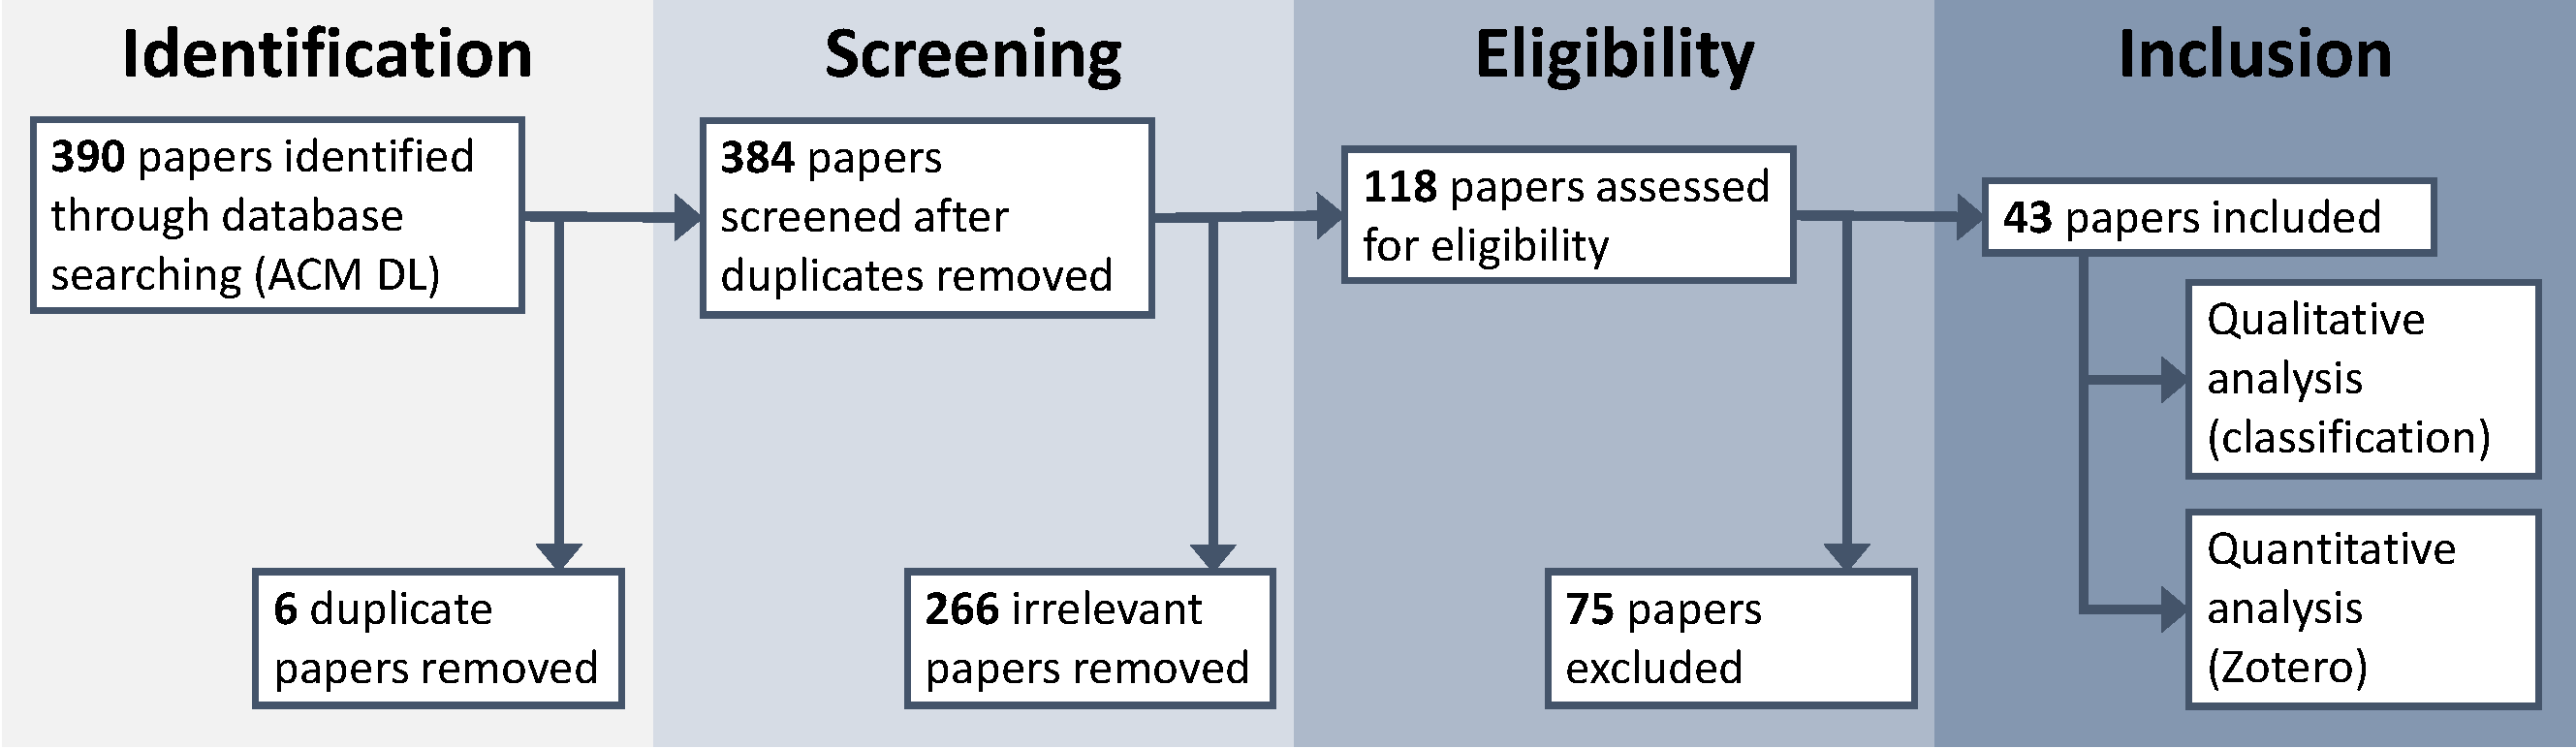
\includegraphics[width=\linewidth]{Figures/StateOfTheArt/LMC/PRISMA-LMC.pdf}
    \vspace{-18pt}
    \captionsetup{width=.9\linewidth}
    \caption{PRISMA diagram~\cite{Page:2021} of our SLR on LMC gesture recognition.}
    \label{fig:state_of_the_art:lmc:prisma}
    % \vspace{-8pt}
\end{figure}

We undertook a Systematic Literature Review (SLR)~\cite{Kitchenham:2010} to explore the algorithms employed for LMC-based gesture recognition (\fig~\ref{fig:state_of_the_art:lmc:prisma}). 
%
The query \texttt{RQ=``leap motion'' AND ``gesture recognition''} was run in the ACM Digital Library\footnote{Accessible at \url{https://dl.acm.org}}, which was highlighted as a good option for computer science literature reviews by Gusenbauer and Haddaway~\cite{Gusenbauer:2020}. Focusing on one extensive database of papers provided us with a good overview of the literature on LMC-based gesture recognition while allowing us to channel most of our efforts into our subsequent SLR on radar-based gesture recognition (Section~\ref{sec:state_of_the_art:radar}).
%
The query yielded 390 publications, from which $N{=}43$ were identified as relevant. 

\subsection{Algorithms} \label{sec:state_of_the_art:lmc:algorithms}
22 types of algorithms for gesture recognition were identified in the papers, spanning across seven categories (\tab~\ref{tbl:state_of_the_art:lmc:algorithms}).

\begin{table}[!b]
    % \resizebox{\columnwidth}{!}{
    \centering
    \footnotesize
    \begin{tabular}{llp{3.1cm}}
        \toprule
        \textbf{Type} & \textbf{Algorithm} & \textbf{References} \\
        \midrule
        Opportunistic & Hard-Coded Thresholds & \cite{Cai:2019,Caputo:2015,Fu:2016,Galea:2018,Sadik:2017,Theofanidis:2017,Tran:2016,Yang:2017,Yao:2017,Yu:2018,Zhou:2018b} \\
         & Leap Gestures & \cite{Caputo:2015,Chatterjee:2015,Daniels:2014,Liang:2017,Mendez:2018,Sadik:2017,Theofanidis:2017,Tran:2016,Yao:2017,Zocco:2015} \\
         & GameWAVE Software & \cite{Liang:2017} \\
        \midrule
        Nearest Neighbor & K-Nearest Neighbors & \cite{Caputo:2017,Chiang:2017,Clark:2016,Daniels:2014,Filho:2018,GomezDonoso:2017,Li:2019,Taranta:2017,Thaweesitthichat:2018,Stinghen:2018} \\
        \midrule
        Support Vector Machines & Support Vector Machine & \cite{Ferreira:2019,Filho:2018,Stinghen:2018,Jiang:2018,Kiselev:2019,Lopez:2015,Marin:2016,Park:2019,Simos:2016} \\
        \midrule
        Neural Networks & Multilayer Perceptron & \cite{Mapari:2016,Togootogtokh:2018} \\
         & Deep Feedforward Neural Network & \cite{Schioppo:2019} \\
         & Feedforward Neural Network & \cite{DePrisco:2016} \\
         & Gated Recurring Units & \cite{Thaweesitthichat:2018} \\
         & Neural Network & \cite{Jiang:2018} \\
         & Radial Basis Function Network & \cite{Zeng:2018} \\
        \midrule
        Hidden Markov Models & Hidden Markov Model & \cite{Kumar:2017a,Kumar:2018,Volioti:2018,Zou:2017} \\
         & Coupled Hidden Markov Model & \cite{Kumar:2017b} \\
        \midrule
        Ensemble Learning & Random Forest & \cite{Marin:2016,Schioppo:2019} \\
         & Bagging Trees & \cite{Jiang:2018} \\
         & Gradient Tree Boosting & \cite{Kiselev:2019} \\
        \midrule
        Other AI/ML Techniques & Decision Tree & \cite{Filho:2018,Stinghen:2018,Zhou:2018b} \\
         & Decision Table & \cite{Li:2017c} \\
         & Linear Discriminant Analysis & \cite{Jiang:2018} \\
         & Fuzzy Integral & \cite{Li:2017c} \\
         & Multinomial Logistic Regression & \cite{Kiselev:2019} \\
         & Naive Bayes & \cite{Preventis:2014} \\
        \bottomrule
    \end{tabular}
    % }
    \caption{Summary of the gesture recognition algorithms identified in the SLR.}
    % \vspace{-20pt}
    \label{tbl:state_of_the_art:lmc:algorithms}
\end{table}

A major part of the analyzed publications ($\frac{16}{43}{=}37\%$) implemented gestural support opportunistically, \ie by relying on the few system-defined gestures natively supported by the LMC or by recognizing gestures based on hard-coded thresholds (\eg \cite{Cai:2019,Galea:2018,Zhou:2018b}). While this opportunistic approach may be appropriate in some cases (\eg for quick prototyping\cite{Anthony:2012} or very simple UIs), it often forces developers to make significant compromises that could be avoided with more advanced recognition techniques. For instance, Liang \etal~\cite{Liang:2017} designed a storytelling system in which children can interact with hand gestures, but these gestures were hard-coded and could not be modified easily to better fit the motor abilities and preferences of each child. Zocco \etal\cite{Zocco:2015} showed that an LMC-based system could be more efficient than the traditional trackpad-keyboard combination to interact with a Command and Control system. However, as they were limited to the few gestures natively supported by the LMC, they did not study whether more suitable types of gestures could result in even greater efficiency and better usability, such as those obtained with user-defined gestures~\cite{Grijincu:2014}.

Found in nine references ($\frac{9}{43}{=}21\%$), K-Nearest Neighbors (KNN) classifiers~\cite{Duda:2000} were also a popular choice for gesture recognition. These algorithms are a simple yet powerful alternative to the opportunistic approach as they are easy to implement and train while being reasonably fast and accurate. Some are presented as all-purpose recognizers \cite{Caputo:2017,Taranta:2017} while others target more specific applications such as handwritten numerals recognition \cite{Chiang:2017} and Sign Language recognition, which remains a key topic for any language: American~\cite{Ferreira:2019,Kumar:2017b,Mapari:2016,Schioppo:2019}, Greek~\cite{Simos:2016}, and Thai~\cite{Thaweesitthichat:2018}.

The remainder of the papers featured more advanced ML techniques such as Neural Networks (NN), SVMs, Hidden Markov Models (HMM), or Ensemble Learning. These techniques were used in all kinds of applications. For instance, Simos and Nikolaos~\cite{Simos:2016} used an SVM to classify the 24 letters of the Greek Sign Language alphabet with high accuracy, and Kumar \etal~\cite{Kumar:2017a} trained an HMM to recognize words from single-stroke Latin sentences.

Among the 27 publications relying exclusively on non-opportunistic algorithms for gesture recognition, only four ($\frac{4}{27}{=}14.8\%$) targeted both static and dynamic gestures, while the rest focused exclusively on one type of gesture.

Finally, some papers combined algorithms and/or sensors. Daniels \etal~\cite{Daniels:2014} combined the LMC's native gestures with Wobbrock \etal's \$1 recognizer~\cite{Wobbrock:2007} to recognize a larger set of gestures for the manipulation of protein structures. Jiang \etal~\cite{Jiang:2018} combined an LMC with myography data, Marin \etal augment the LMC with an MS Kinect~\cite{Marin:2014} or a depth sensor~\cite{Marin:2016} to increase accuracy. 

%--------------------------------------------------------------------------------%
\subsection{Summary} \label{sec:state_of_the_art:lmc:summary}
Despite the popularity and ease of use of the LMC, we observe that none of the papers discussed in the previous section attempted to propose an approach that is reusable across gesture sets, gestural UIs, and applications towards their mainstream development. Reusability, interoperability, and maintainability, three important (sub-)factors for software quality defined in the ISO/IEC 25010~\cite{iso25010}, are not explicitly addressed.


%================================================================================%
\section{A Deep Dive into Radar-based Gesture Interaction} \label{sec:state_of_the_art:radar}

To get a comprehensive look at the state of the research on radar-based gesture interaction, an SLR was conducted to identify the types of radar, algorithms, and gesture sets used for radar-based gesture recognition (\fig~\ref{fig:state_of_the_art:radar:prisma}). The query \texttt{RQ=``radar'' AND ``gesture recognition''} was run in five digital libraries: (1) \href{https://dl.acm.org/}{ACM Digital Library}, (2) \href{https://ieeexplore.ieee.org/Xplore/home.jsp}{IEEE Xplore}, (3) \href{https://www.mdpi.com/journal/sensors}{MDPI (Sensors)}, (4) \href{https://link.springer.com/}{SpringerLink}, and (5) \href{https://www.sciencedirect.com/}{Elsevier ScienceDirect} and resulted in 1,515 articles, from which $N=118$ were identified as relevant. \tab~\ref{tab:state_of_the_art:radar-slr-references} groups these papers based on their year of publication. 91.5\% of the papers were published between 2018 and 2020, indicating that this field of research has recently become quite active. 

\begin{figure}[hbt]
    \centering
    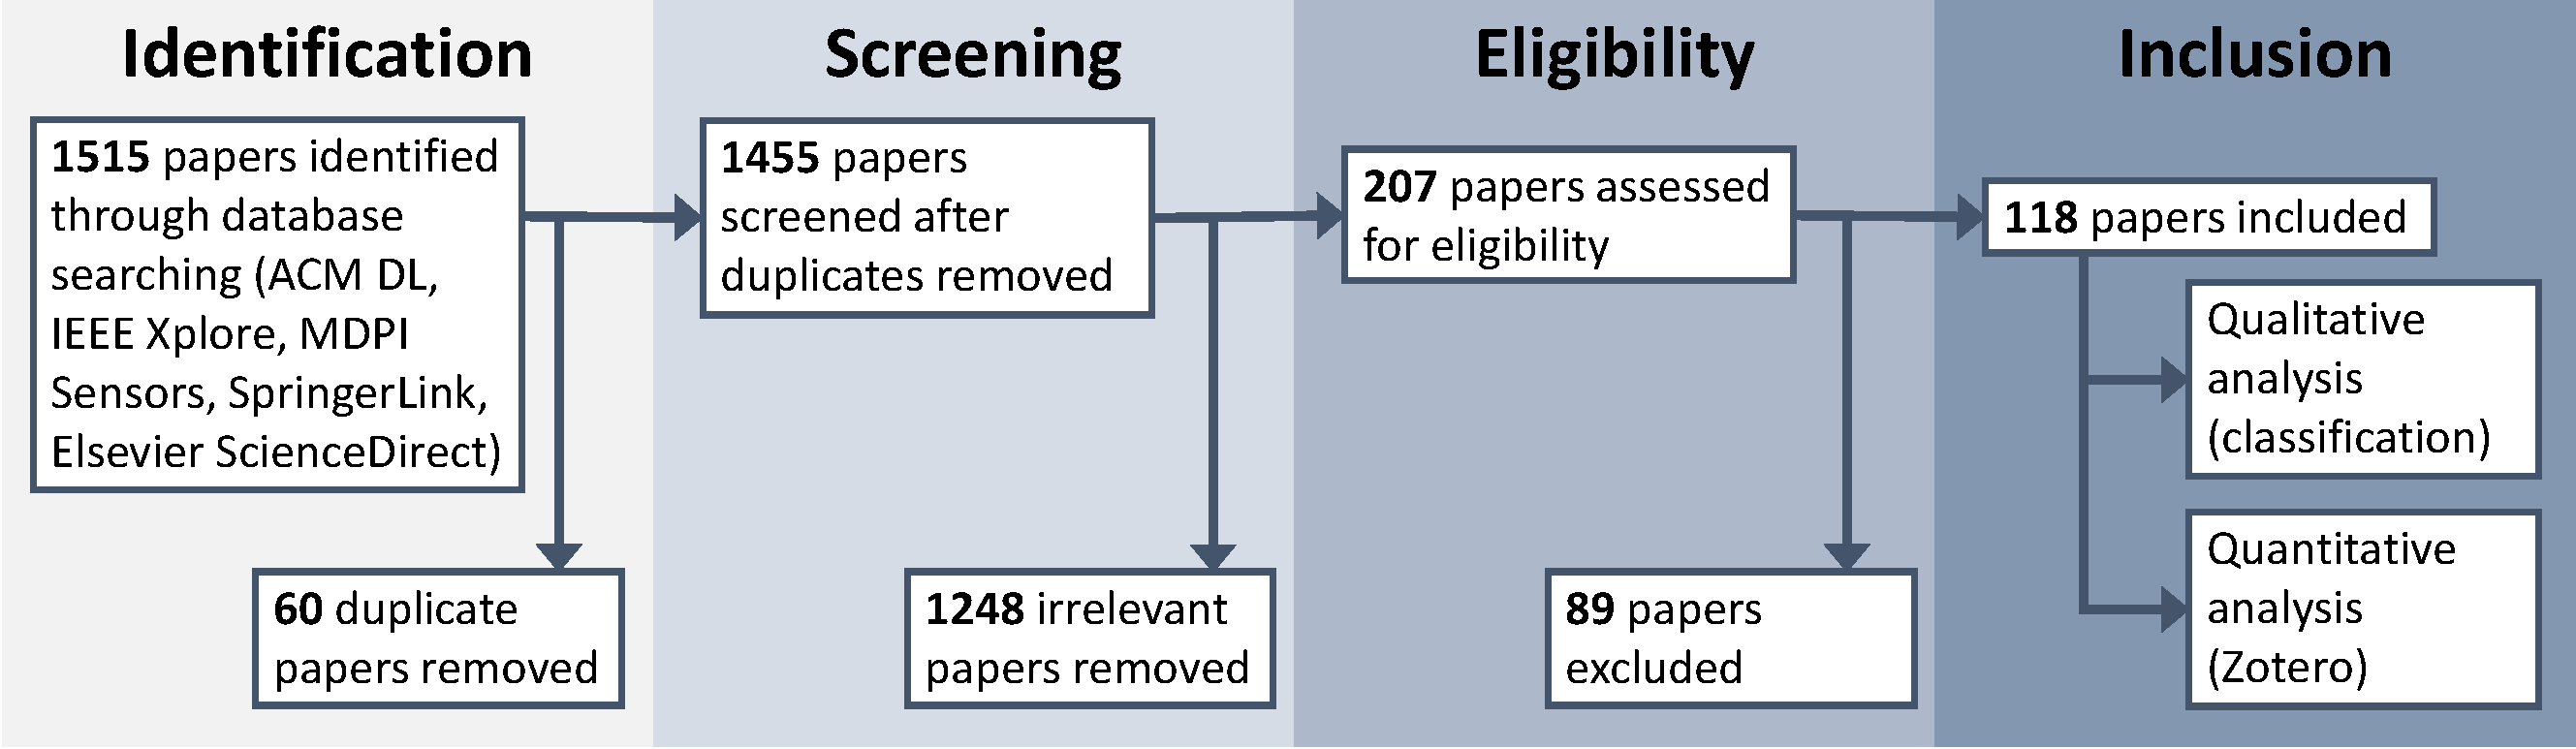
\includegraphics[width=\linewidth]{Figures/StateOfTheArt/Radar/PRISMA-Radar.pdf}
    % \vspace{-18pt}
    \caption{PRISMA diagram~\cite{Page:2021} of our SLR on radar-based gesture interaction.}
    \label{fig:state_of_the_art:radar:prisma}
    % \vspace{-8pt}
\end{figure}

\begin{table}[t]
    \centering
    \footnotesize
    \begin{tabular}{crp{.78\textwidth}}
        \toprule
        \textbf{Year} & \textbf{\#Refs} & \textbf{Reference(s)} \\
        \midrule
        2009 & 1 & \cite{Li:2009} \\
        2014 & 1 & \cite{Wan:2014} \\
        2015 & 1 & \cite{Molchanov:2015} \\
        2016 & 6 & \cite{Kim:2016,Lien:2016,Malysa:2016,Park:2016,Wang:2016,Zhang:2016} \\
        2017 & 11 & \cite{Lan:2017,Li:2017a,Mcintosh:2017,Ritchie:2017,Sakamoto:2017,Viunytskyi:2017,Zhang:2017,Kim:2017b,Kim:2017a,Dekker:2017,Khan:2017} \\
        2018 & 21 & \cite{Hazra:2018,Ishak:2018,Lan:2018b,Lan:2018a,Li:2018b,Li:2018a,Lou:2018,Nguyen:2018a,Nguyen:2018b,Patra:2018,Ryu:2018,Sakamoto:2018,Smith:2018,Suh:2018,Sun:2018,Yang:2018,Zhang:2018d,Zhang:2018a,Zhang:2018b,Zhang:2018c,Zhou:2018a} \\
        2019 & 35 & \cite{Ahmed:2019,Amin:2019b,Amin:2019a,Arsalan:2019,Arthamanolap:2019,Berenguer:2019,Chen:2019,Choi:2019,Copic:2019,Du:2019,Eggimann:2019,Ehrnsperger:2019,Feng:2019,Fhager:2019,Ghaffar:2019,Gigie:2019,Goswami:2019,Hazra:2019b,Hazra:2019a,Kang:2019,Kulhandjian:2019,Liu:2019,Skaria:2019,Sun:2019,Wang:2019f,Wang:2019a,Wang:2019b,Wang:2019c,Wang:2019d,Wang:2019e,Zhang:2019d,Zhang:2019a,Zhang:2019b,Zhang:2019c,Zhao:2019} \\
        2020 & 41 & \cite{Ahmed:2020,Amin:2020,Bannon:2020,Du:2020,Ehrnsperger:2020,Gurbuz:2020,Kern:2020,Khan:2020,Lee:2020,Leem:2020b,Leem:2020a,Li:2020b,Li:2020a,Liang:2020,Liu:2020b,Liu:2020a,Miller:2020,Park:2020,Ren:2020,Ritchie:2020,Rozman:2020,Santhalingam:2020b,Santhalingam:2020a,Skaria:2020b,Skaria:2020a,Sun:2020b,Sun:2020a,Tzadok:2020,Vandersmissen:2020,Wang:2020d,Wang:2020a,Wang:2020b,Wang:2020c,Wu:2020,Xia:2020,Yu:2020b,Yu:2020a,Zeng:2020b,Zeng:2020a,Zhang:2020b,Zhang:2020a} \\
        2021 & 1 & \cite{Ahmad:2021} \\
        \bottomrule
    \end{tabular}
    \caption{Distribution of papers from our systematic literature review, based on their year of publication.}
    \label{tab:state_of_the_art:radar-slr-references}
    % \vspace{-14pt}
\end{table}

%--------------------------------------------------------------------------------%
\subsection{Applications} \label{sec:state_of_the_art:radar:applications}
While all papers provided some evaluation of the system performance (see \fig~\ref{fig:state_of_the_art:radar:validation-type}), only 14 papers ($\frac{14}{118}{=}12\%$) demonstrated potential use cases of their system with a prototype and one paper ($\frac{1}{118}{=}1\%$) evaluated the user experience of the proposed system.

\begin{figure}[t]
    \centering
    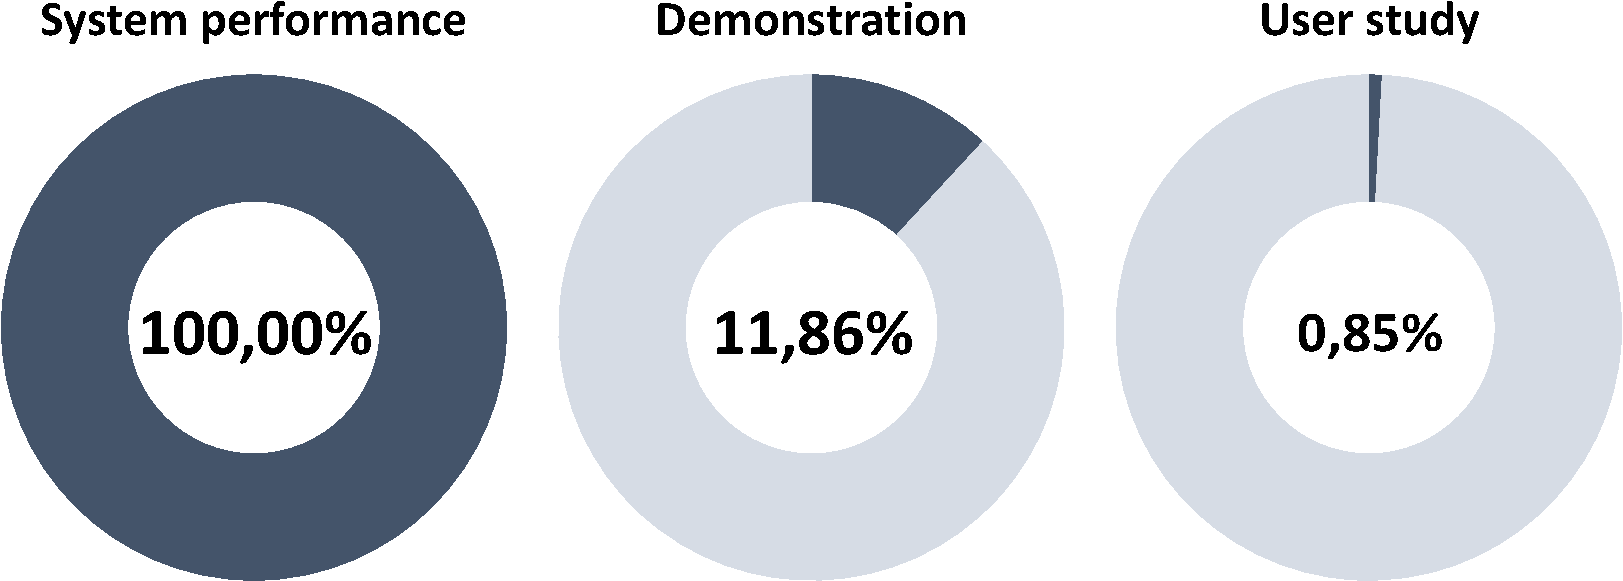
\includegraphics[height=2.6cm]{Figures/StateOfTheArt/Radar/evaluation-type.pdf}
    % \vspace{-10pt}
    \caption{Types of validation.}
    \label{fig:state_of_the_art:radar:validation-type}
%    \vspace{-6pt}
\end{figure}


Eight of the 14 papers focused on multimedia applications, including controlling media playback (\eg music, videos)~\cite{Du:2019,Lee:2020,Wu:2020,Smith:2018,Liu:2020b} or triggering specific keystrokes (\eg Enter, Alt+F4)~\cite{Nguyen:2018a,Nguyen:2018b}, thus enabling the control of classical PC applications without modifications to their source code.
Liu \etal~\cite{Liu:2020b} introduced \textit{mHomeGes}, a radar-based gesture recognition system for smart homes that allowed users to control lighting, music, and a home monitor. After evaluating the user experience of the system, the authors observed that 70\% of the users found \textit{mHomeGes} more convenient than voice commands.
Smith \etal~\cite{Smith:2018} implemented in-vehicle interaction for the driver and passengers of a car to control music and answer phone calls.
Lien \etal~\cite{Lien:2016} introduced \textit{virtual tookits}, \ie small sets of gestures complex enough to enable the control of UIs while being memorable and easy for the system to recognize. They built a pipeline based on the Google Soli radar to recognize gestures in real-time and trigger actions in applications accordingly.
Wu \etal~\cite{Wu:2020} proposed to embed radar antennas into fabric to augment everyday objects (\eg furniture, clothing) with gesture-based interfaces. The authors developed prototypes to demonstrate various use cases, including controlling media playback with an interactive sofa armrest, checking fitness goals with interactive sports clothing, and creating interactive plush toys.

Other applications included air-writing recognition~\cite{Wang:2020a}, user authentication based on 2D hand trajectories and breathing patterns~\cite{Leem:2020b}, making a home-assistant for people with hearing impairements~\cite{Santhalingam:2020b}, manipulating medical images in an operating room~\cite{Miller:2020}, and controlling a robot with hand gestures~\cite{Zhang:2020a,Li:2009}.

%--------------------------------------------------------------------------------%
\subsection{Algorithms} \label{sec:state_of_the_art:radar:algorithms}

\fig~\ref{fig:state_of_the_art:radar:algorithms} presents the algorithms used in our corpus.
151 algorithms for radar-based gesture recognition were identified, the majority representing deep learning approaches ($\frac{81}{151}=54\%$), of which Convolutional Neural Networks (CNN) were the most frequently used.
CNNs were often combined with other models, such as Long Short-Term Memory (LSTM) or SVMs, in $\frac{23}{158}=15\%$ of the cases.
Classical machine learning algorithms were still used, as follows: K Nearest Neighbors ($\frac{23}{151}=15\%$), Support Vector Machines ($\frac{16}{151}=11\%$), ensemble learning ($\frac{8}{151}=5\%$), Decision Trees ($\frac{6}{151}=4\%$), Hidden Markov Models ($\frac{3}{151}=2\%$), and Bayesian networks ($\frac{2}{151}=1\%$). 

\begin{figure}[t]
    \centering
    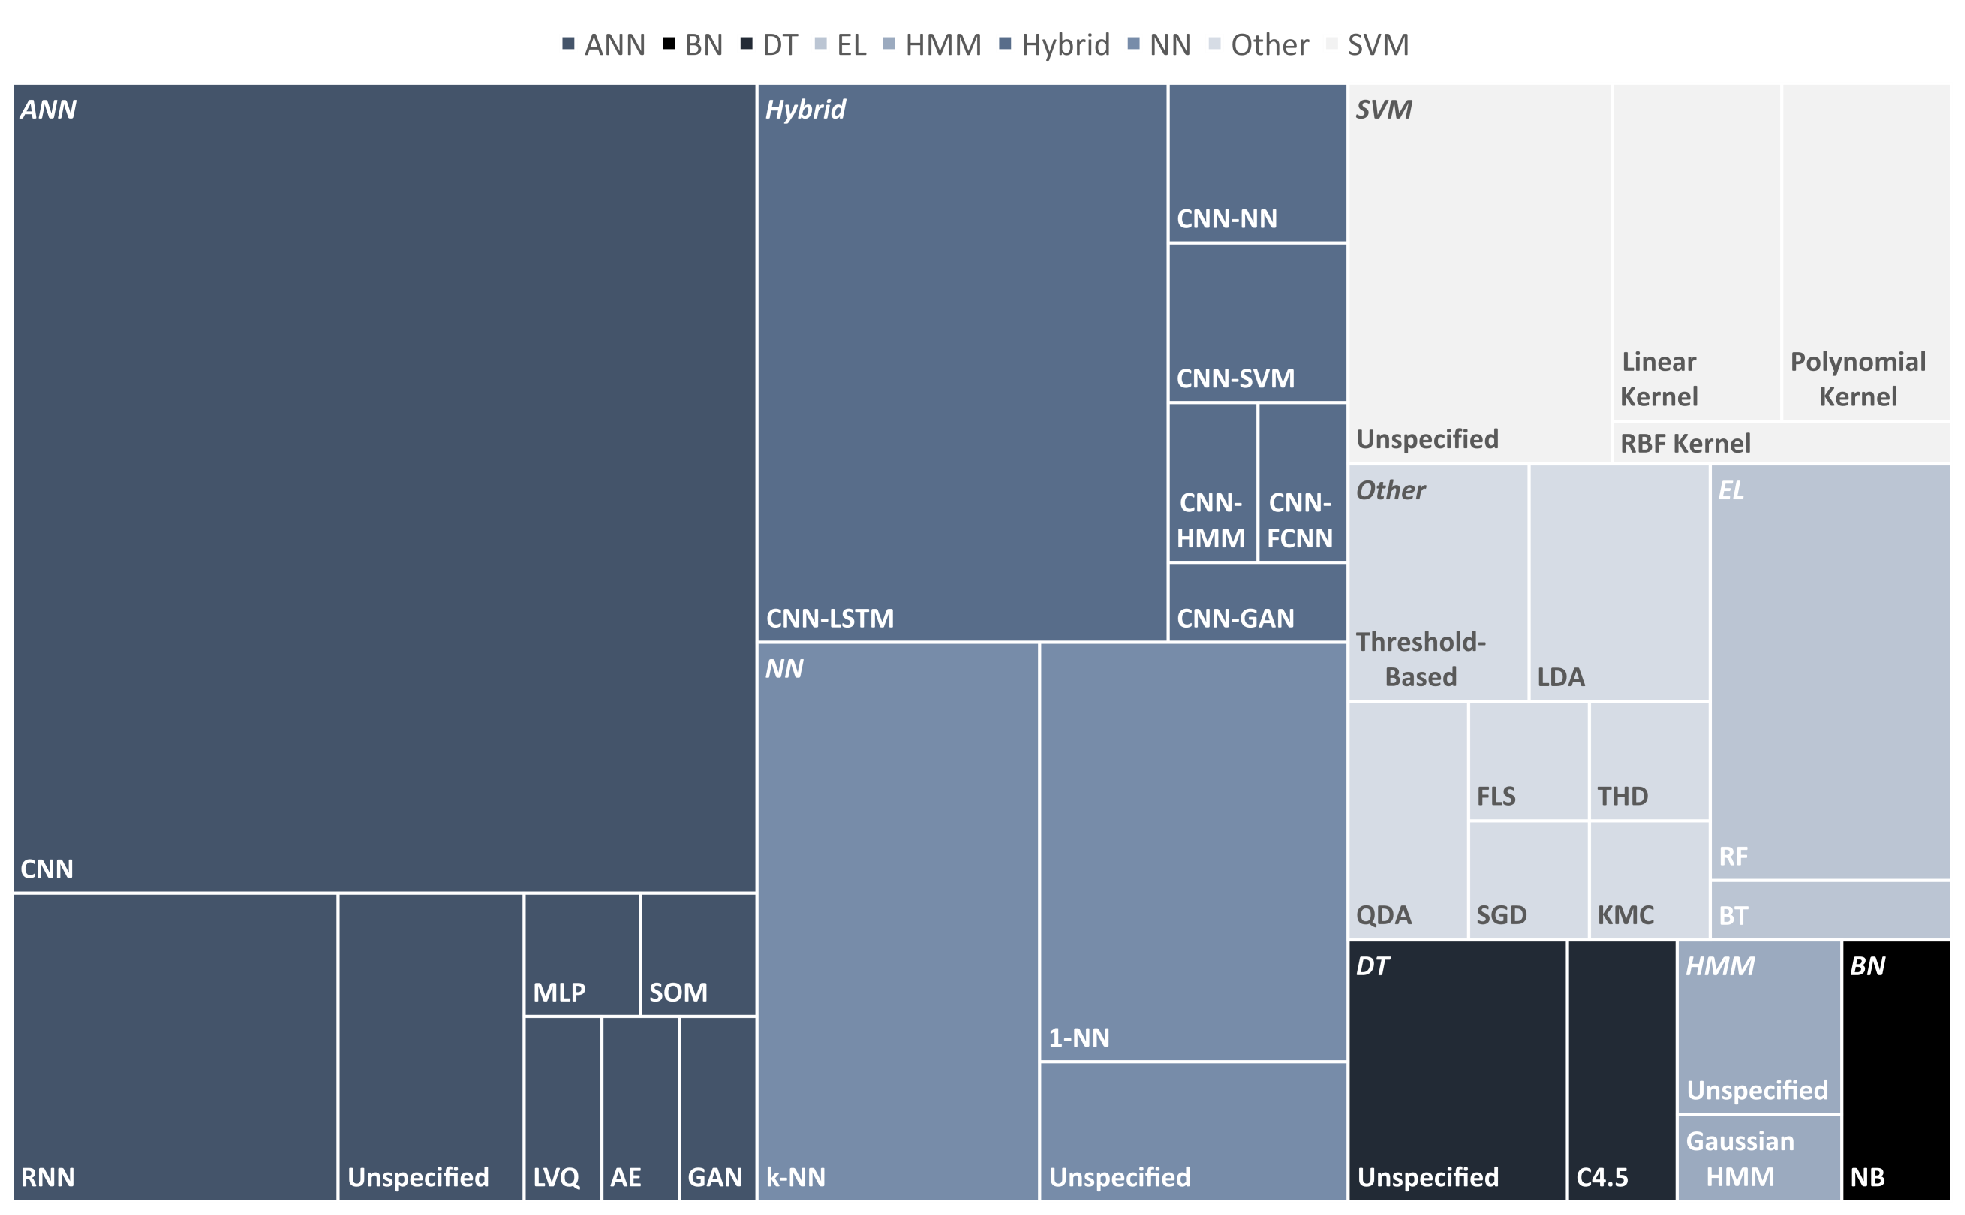
\includegraphics[width=\linewidth]{Figures/StateOfTheArt/Radar/treemap-algorithms.pdf}
    \vspace{-10pt}
    \caption{Tree map~\cite{Shneiderman:1992} of the algorithms for radar-based gesture recognition identified in the corpus. The color of a cell indicates the type of algorithm (\eg ANN, HMM, or SVM) while the size of a cell is proportional to the number of papers featuring this algorithm.}
    \label{fig:state_of_the_art:radar:algorithms}
%    \vspace{-6pt}
\end{figure}


From the above analysis, we make the following observations
\begin{enumerate}
    \item \textit{Predominance of CNN algorithms}: CNNs, often coupled with other models like LSTMs, are predominant for recognizing radar-based signals. They are particularly appropriate for image processing, but also they benefit from their intrinsic capability to select the discriminant radar features without any human supervision. This ability proves particularly useful when dealing with gesture sets that are very large in size and complexity, as radar images are very challenging to discriminate by a non-expert.
    %
    An alternative to relying on CNNs for feature selection involves extracting point clouds from raw radar signals and directly inputting them into a classification algorithm, such as an LSTM~\cite{Palipana:2021}. This approach can be more efficient thanks to the smaller size of point clouds compared to raw radar data.
    \item \textit{Dependence of CNN with respect to the radar}: since CNNs automatically select features directly from radar images, these key features are not pre-trained and only learned when the gesture set is examined, thereby making the CNN very appropriate, but also very specific to the radar images produced. The CNNs therefore suffer from a high dependence on radar type and possibly radar unit for a given model. 
    \item \textit{No modeling of the radar functioning}: since CNNs ensure most of the work for a specific radar, we did not identify any work in gesture recognition aimed at modeling the radar functioning in some way to ensure some radar independence or some mechanism to reason about its processing. 
\end{enumerate}



%--------------------------------------------------------------------------------%
\subsection{Gestures} \label{sec:state_of_the_art:radar:gestures}

\begin{figure}[t]
    \centering
    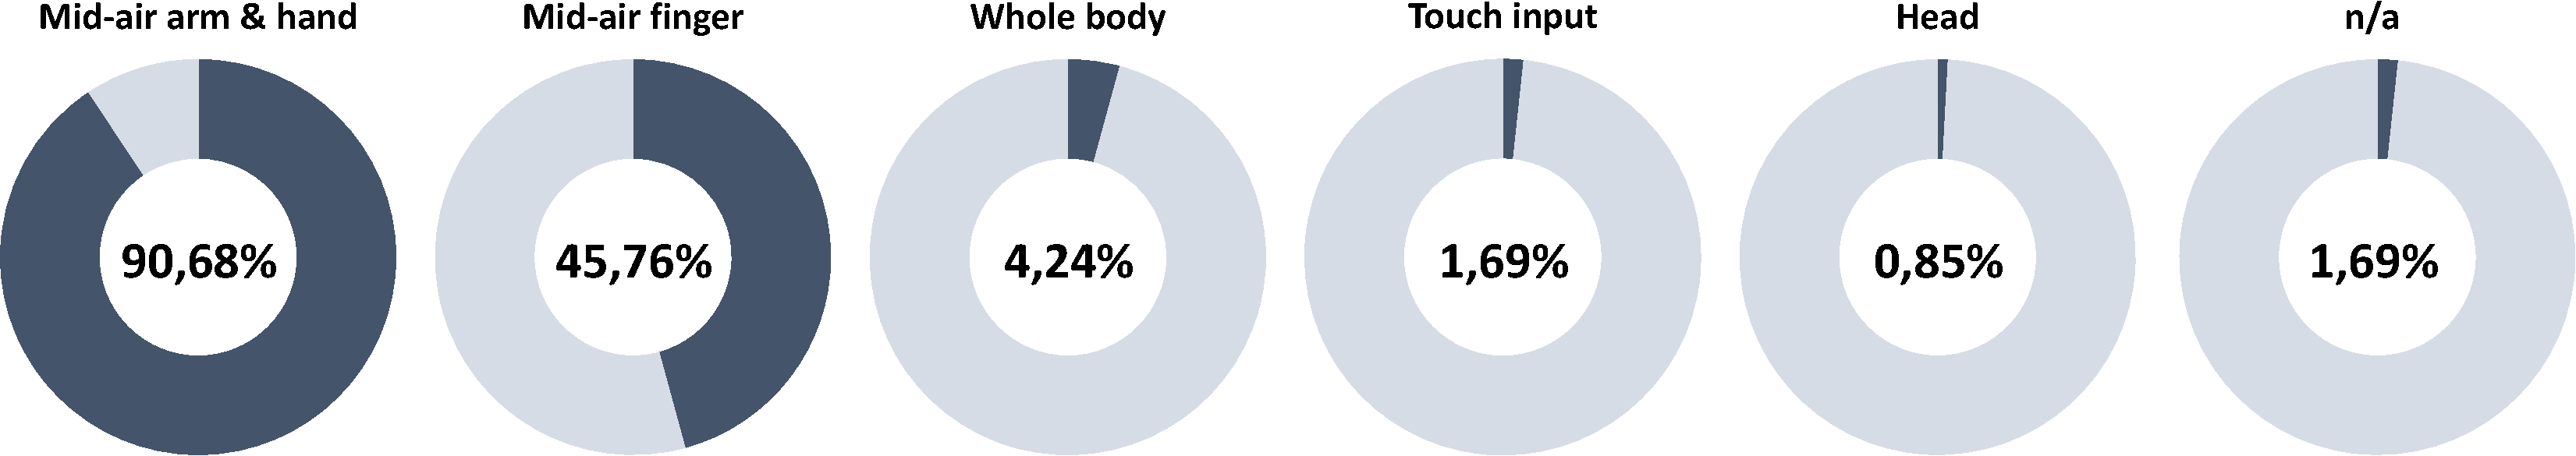
\includegraphics[width=\linewidth]{Figures/StateOfTheArt/Radar/gestures-type.pdf}
    % \vspace{-10pt}
    \caption{Types of gestures.}
    \label{fig:state_of_the_art:radar:gestures-type}
%    \vspace{-6pt}
\end{figure}


\fig~\ref{fig:state_of_the_art:radar:gestures-type} gives an overview of the types of gestures used in the identified papers. Most papers ($\frac{107}{118}=91\%$) featured mid-air arm and hand gestures, which are relatively easy to recognize thanks to their scale that is neither too small, thus not requiring extremely fine range resolution, nor too large, which makes it possible for the radar to focus exclusively on the current user, thus simplifying signal processing. Almost half of the papers ($\frac{54}{118}=46\%$) featured mid-air finger gestures, which require higher frequency radars (capable of finer range resolution) to accurately capture the fine-grained finger motion. Other papers featured whole body gestures~\cite{Li:2009,Li:2020b,Vandersmissen:2020}, touch input~\cite{Copic:2019,Wu:2020}, or even head gestures~\cite{Wan:2014}.
%
We identified only seven publicly available datasets out of the 118 papers from our SLR; see \tab~\ref{tab:state_of_the_art:radar-slr-datasets}. 
The mHomeGes dataset~\cite{Liu:2020b} comprises 10 types of arm gestures collected from 25 participants: arm up/down, push, pull, draw a circle, draw a zigzag, clap hands, mimic knocking on a table, yawn, and lift both arms. Each gesture was recorded in seven environments, including a bedroom and a parlor.
\cite{Santhalingam:2020b} collected 50 different ASL signs from 15 participants in three environments (classroom, laboratory, and conference room) and five different scenarios for single and multiple users. Data were recorded simultaneously with a radar, a Kinect, and an RGB camera.
%
Deep-soli is a dataset introduced by \cite{Wang:2016} that comprises 11 hand gestures performed by 10 users above Google Soli: pinch index/pinky, finger slide, finger rub, slow/fast swipe, push, pull, palm tilt, circle, and palm hold. Deep-Soli was also used by \cite{Berenguer:2019} to evaluate GestureVLAD, their proposed framework for radar gesture recognition.
%
\cite{Ritchie:2020} introduce Dop-net, a dataset of four gestures recorded with two different radar sensors (CW and FMCW). Only the FMCW dataset was released in the form of a challenge. Dop-net was used in another paper to compare the performance of CW and FMCW radars for gesture recognition~\cite{Bannon:2020}.
%
Finally, HARrad consists of two datasets of six gestures of arm and hand gestures collected from nine participants with a 77GHz radar~\cite{Vandersmissen:2020}: drumming, shaking, swiping left/right, and thumb up/down. HARrad events contain six different actions, including entering or leaving a room, sitting down, standing up, getting dressed, and undressing.

From the above analysis, we make the following observations:
\begin{enumerate}
\setcounter{enumi}{3}
    \item \textit{Limited availability of datasets}: very little datasets are available for benchmarking.
    \item \textit{Huge size of datasets}: the size of the raw data captured for a single gesture is very high, making the entire dataset huge in size and challenging to process. Little or no dimension reduction has been observed.
\end{enumerate}

%--------------------------------------------------------------------------------%
\subsection{Radars} \label{sec:state_of_the_art:radar:sensors}

\begin{table}[!b]
    \centering
    %\vspace{-8pt}
    \footnotesize
    \begin{tabular}{>{\raggedright}p{1.8cm}rrr>{\raggedright}p{2.6cm}>{\raggedright}p{0.8cm}>{\raggedright\arraybackslash}p{0.9cm}}
        \toprule
        \textbf{Name} & \textbf{Classes} & \textbf{Users} & \textbf{Samples} & \textbf{Sensor(s)} & \textbf{Base paper} & \textbf{Other papers} \\
        \midrule
        mHomeGes & 10 & 25 & $>$22000 & TI IWR1443 & \cite{Liu:2020b} & /  \\
        \addlinespace[2pt]
        mmASL (wake-words) & 2 & 3 & 3700 & NI multi-FPGA platform (w/ NI PXIe7902, 7976, 3610/3630) and SiBeam phased antenna array & \cite{Santhalingam:2020b} & /  \\
        \addlinespace[2pt]
        mmASL (signs) & 50 & 15 & 12236 & NI multi-FPGA platform (w/ NI PXIe7902, 7976, 3610/3630) and SiBeam phased antenna array + Kinect + RGB camera  & \cite{Santhalingam:2020b} & /  \\
        \addlinespace[2pt]
        deep-soli & 11 & 11 & 5500 & Google Soli & \cite{Wang:2016} & \cite{Berenguer:2019}  \\
        \addlinespace[2pt]
        dop-net & 4 & 6 & 3052 & Ancortek SDR-KIT 2400AD2 & \cite{Ritchie:2020} & \cite{Bannon:2020}  \\
        \addlinespace[2pt]
        HARrad\newline(gestures) & 6 & 9 & 2347 & 77GHz FMCW radar & \cite{Vandersmissen:2020} & /  \\
        \addlinespace[2pt]
        HARrad (events) & 6 & 9 & 1505 & 77GHz FMCW radar & \cite{Vandersmissen:2020} & /  \\
        \bottomrule
    \end{tabular}
    \caption{Summary of the publicly available datasets identified in our systematic literature review.}
    \label{tab:state_of_the_art:radar-slr-datasets}
%   \vspace{-14pt}
\end{table}

We identified 123 radar systems and extracted their parameters, including the radar type, the frequency band in which they operate, the model, and their position. We identified four types of radars (\fig~\ref{fig:state_of_the_art:radar:types}): 
\begin{itemize}
    \item \textit{Frequency-Modulated Continuous-Wave} (FMCW) radars ($\frac{65}{123}{=}53\%$), which continuously transmit a signal that varies in frequency, \ie modulated in frequency. These radars can resolve both the range and Doppler~\cite{AlHourani:2018}, enabling the recognition of static poses and dynamic gestures.
    
    \item \textit{Unmodulated Continuous-Wave} (CW) radars ($\frac{36}{123}{=}29\%$), which continuously transmit a signal at a constant frequency and amplitude~\cite{Oberhammer:2013}. These radars are simple and inexpensive. They can measure the Doppler shift of the return signal caused by moving objects but cannot provide range information or identify stationary targets, as the latter do not cause a Doppler shift. Consequently, radars of this type are not suitable for detecting static poses of the hand or body.
    
    \item \textit{Pulse} radars ($\frac{21}{123}{=}17\%$) transmit short radar pulses and listen for the returning echo. These radars can measure the range of targets, stationary and moving, making them suitable for the recognition of static poses and dynamic gestures. The pulse length affects the radar detection range (a longer pulse length increases the maximum range but may prevent the detection of very close targets) as well as its range resolution (a shorter pulse length allows for better discrimination between two spatially separated targets)~\cite{Bole:2014}. The smaller the pulse length in the time domain, the larger the bandwidth in the frequency domain counterpart.
    
    \item  \textit{Direct-Sequence Spread Spectrum} (DSSS) radars ($\frac{1}{123}{=}1\%$)  transmit signals modulated by a random bit sequence. These radars can measure the range of stationary and moving targets, and their architecture is simpler than FMCW radars~\cite{Tang:2020}.
\end{itemize}

\begin{figure}[t]
    \begin{subfigure}{.49\textwidth}
        \centering
        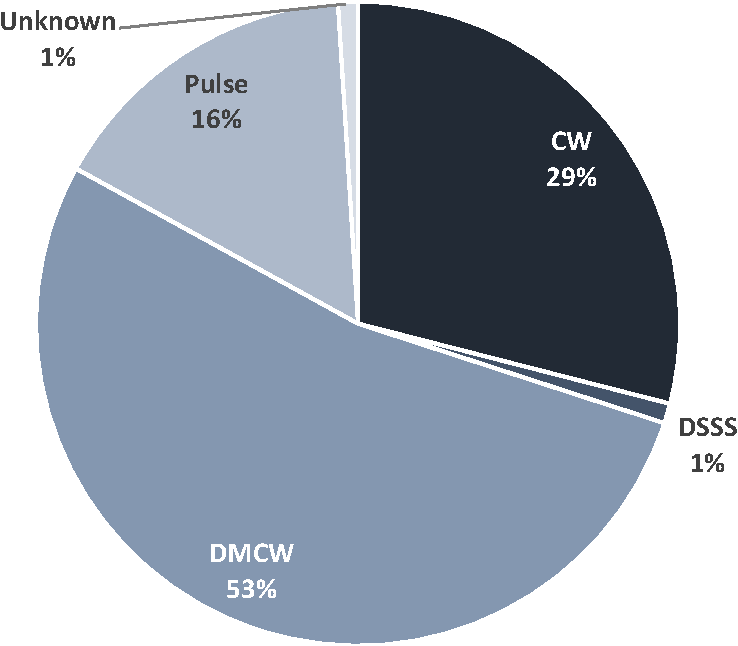
\includegraphics[height=.75\linewidth]{Figures/StateOfTheArt/Radar/radar-types.pdf}
        % \vspace{-6pt}
        \captionsetup{width=.9\linewidth}
        \caption{Radar type.}
        \label{fig:state_of_the_art:radar:types}
    \end{subfigure}
    \begin{subfigure}{.49\textwidth}
        \centering
        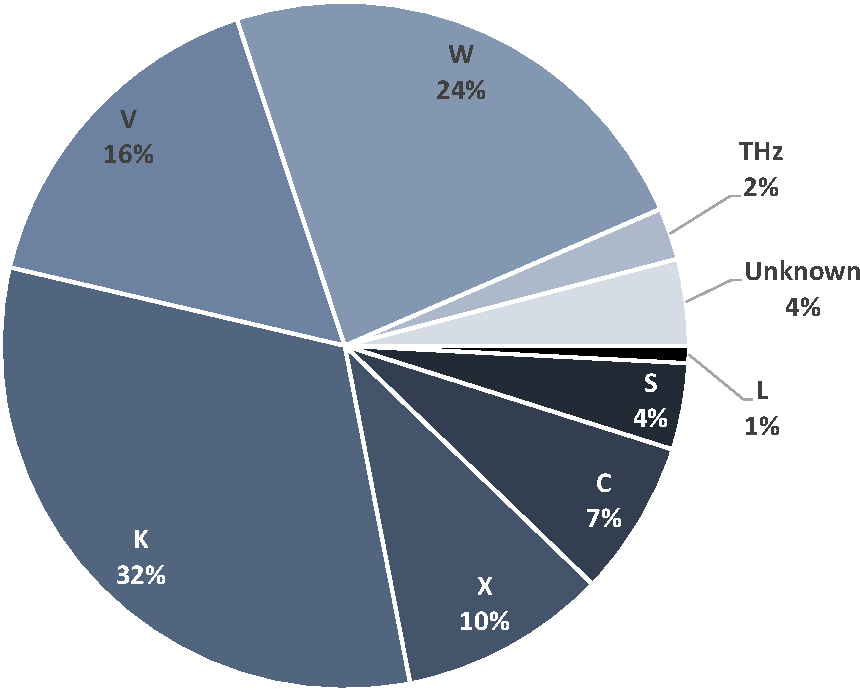
\includegraphics[height=.75\linewidth]{Figures/StateOfTheArt/Radar/radar-frequencies.pdf}  
        % \vspace{-6pt}
        \captionsetup{width=.9\linewidth}
        \caption{Frequency band~\cite{IEEE:2020}.}
        \label{fig:state_of_the_art:radar:frequencies}
    \end{subfigure}
    \caption{Distribution of the radars identified in our systematic literature review.}
    \label{fig:state_of_the_art:radar:pie-charts}
    % \vspace{-8pt}
\end{figure}
%The type of one radar ($\frac{1}{123}{=}1\%$) could not be identified. 
Most of the papers ($\frac{98}{118}{=}83\%$) relied on a single radar sensor to capture gestures, while the rest ($\frac{20}{118}{=}17\%$) used two or more radars. Among the latter, four papers introduced different radar models. Some papers introduced other types of sensors, such as~\cite{Santhalingam:2020b}, where gestures were collected using a radar, a Kinect, and an RGB camera for comparison purposes. \cite{Gigie:2019} synthesized micro-Doppler radar signatures of gestures from the skeleton provided by a Kinect. Other papers performed data fusion with RGB cameras~\cite{Molchanov:2015,Vandersmissen:2020}, depth cameras~\cite{Tzadok:2020,Molchanov:2015}, and thermal cameras~\cite{Skaria:2020b}, respectively.

\fig~\ref{fig:state_of_the_art:radar:radar-position} summarizes the position of the radar systems identified in the user environment. Almost half of the identified papers ($\frac{49}{118} = 42\%$) did not provide enough information about the position of the radar(s) in the user's environment. From the papers that provided this information, 47 ($\frac{47}{118} = 40\%$) placed the radar(s) on a table, while 10 ($\frac{10}{118} = 8\%$) placed them on a tripod, and six ($\frac{6}{118} = 5\%$) in the car (\eg on the center console~\cite{Molchanov:2015}, near the steering wheel~\cite{Ahmed:2019, Sun:2018}, or on the roof console~\cite{Sun:2019}). Other positions include on the body~\cite{Miller:2020,Copic:2019}, on fabric~\cite{Wu:2020}, and on a robot~\cite{Li:2009}.

\begin{figure}[t]
    \centering
    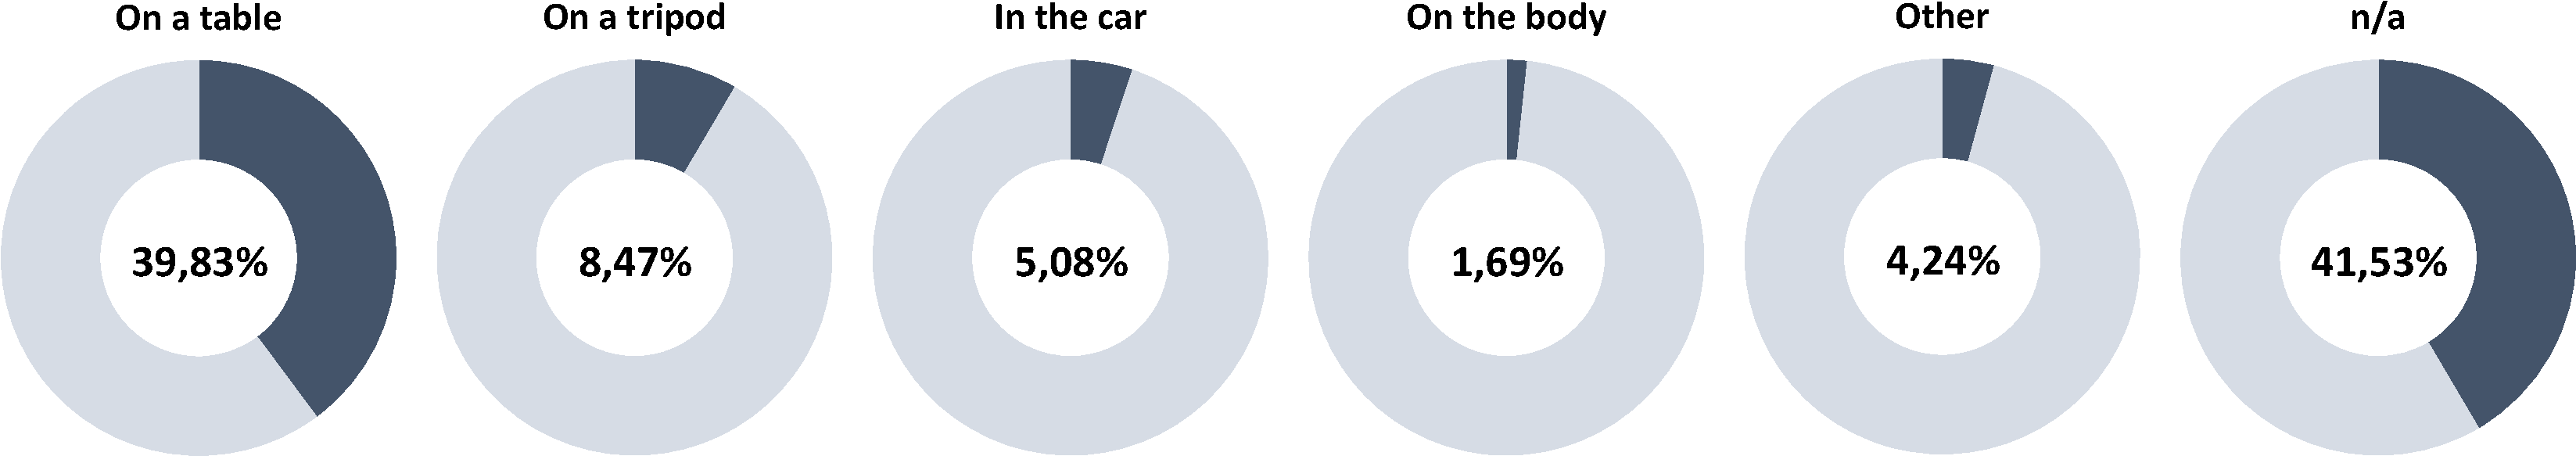
\includegraphics[width=\linewidth]{Figures/StateOfTheArt/Radar/radar-positions.pdf}
    % \vspace{-10pt}
    \caption{Positions of the radar.}
    \label{fig:state_of_the_art:radar:radar-position}
%    \vspace{-6pt}
\end{figure}

\begin{figure}[t]
    \centering
    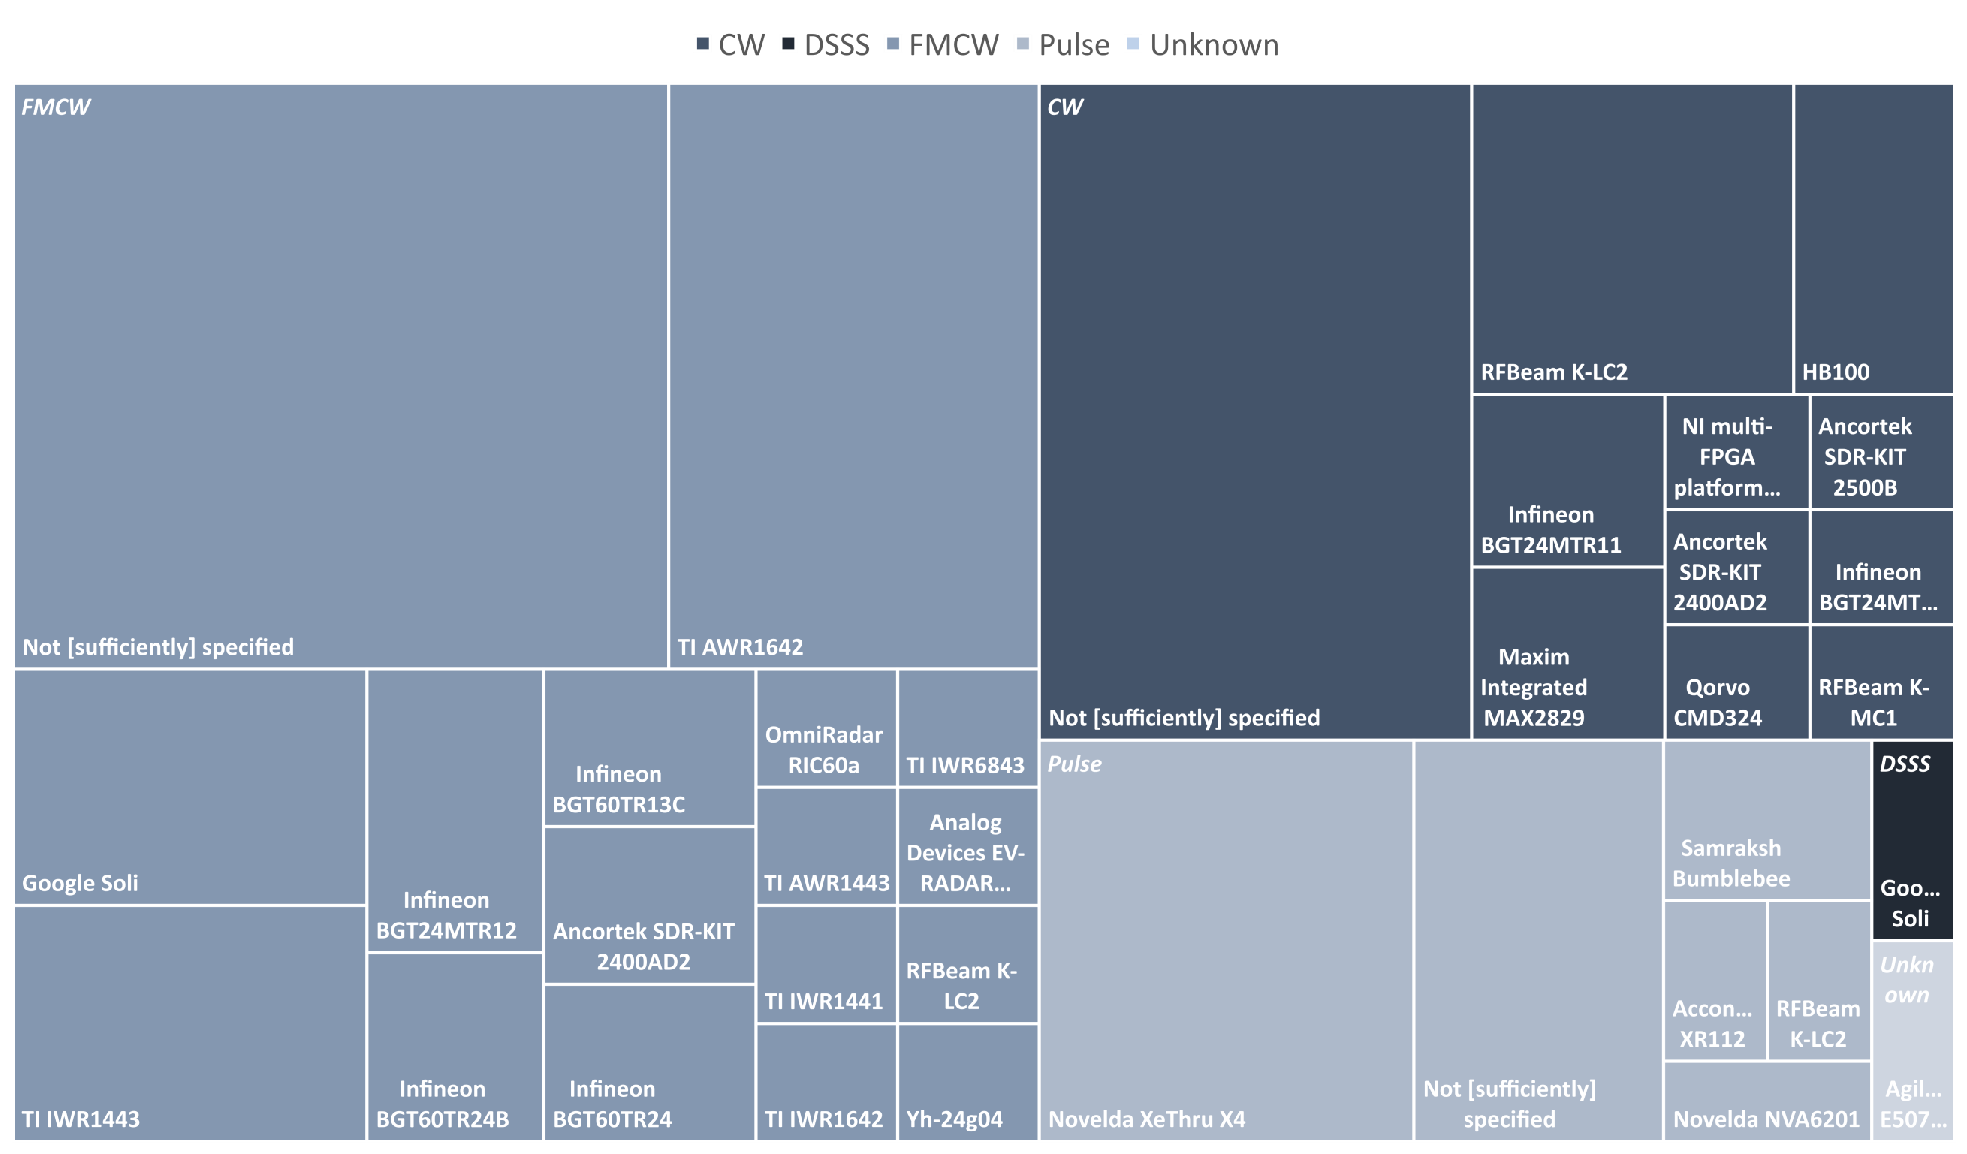
\includegraphics[width=\linewidth]{Figures/StateOfTheArt/Radar/treemap-radar-types-models.pdf}
    \vspace{-16pt}
    \caption{Tree map~\cite{Shneiderman:1992} of the radar models identified in our systematic literature review. 
    The color of a cell indicates the type of radar (CW, DSSS, FMCW, Pulse, or unknown) while the size of a cell is proportional to the number of papers featuring this model of radar.}
    \label{fig:state_of_the_art:radar:radars}
    %\vspace{-8pt}
\end{figure}

\begin{figure}[t]
    \centering
    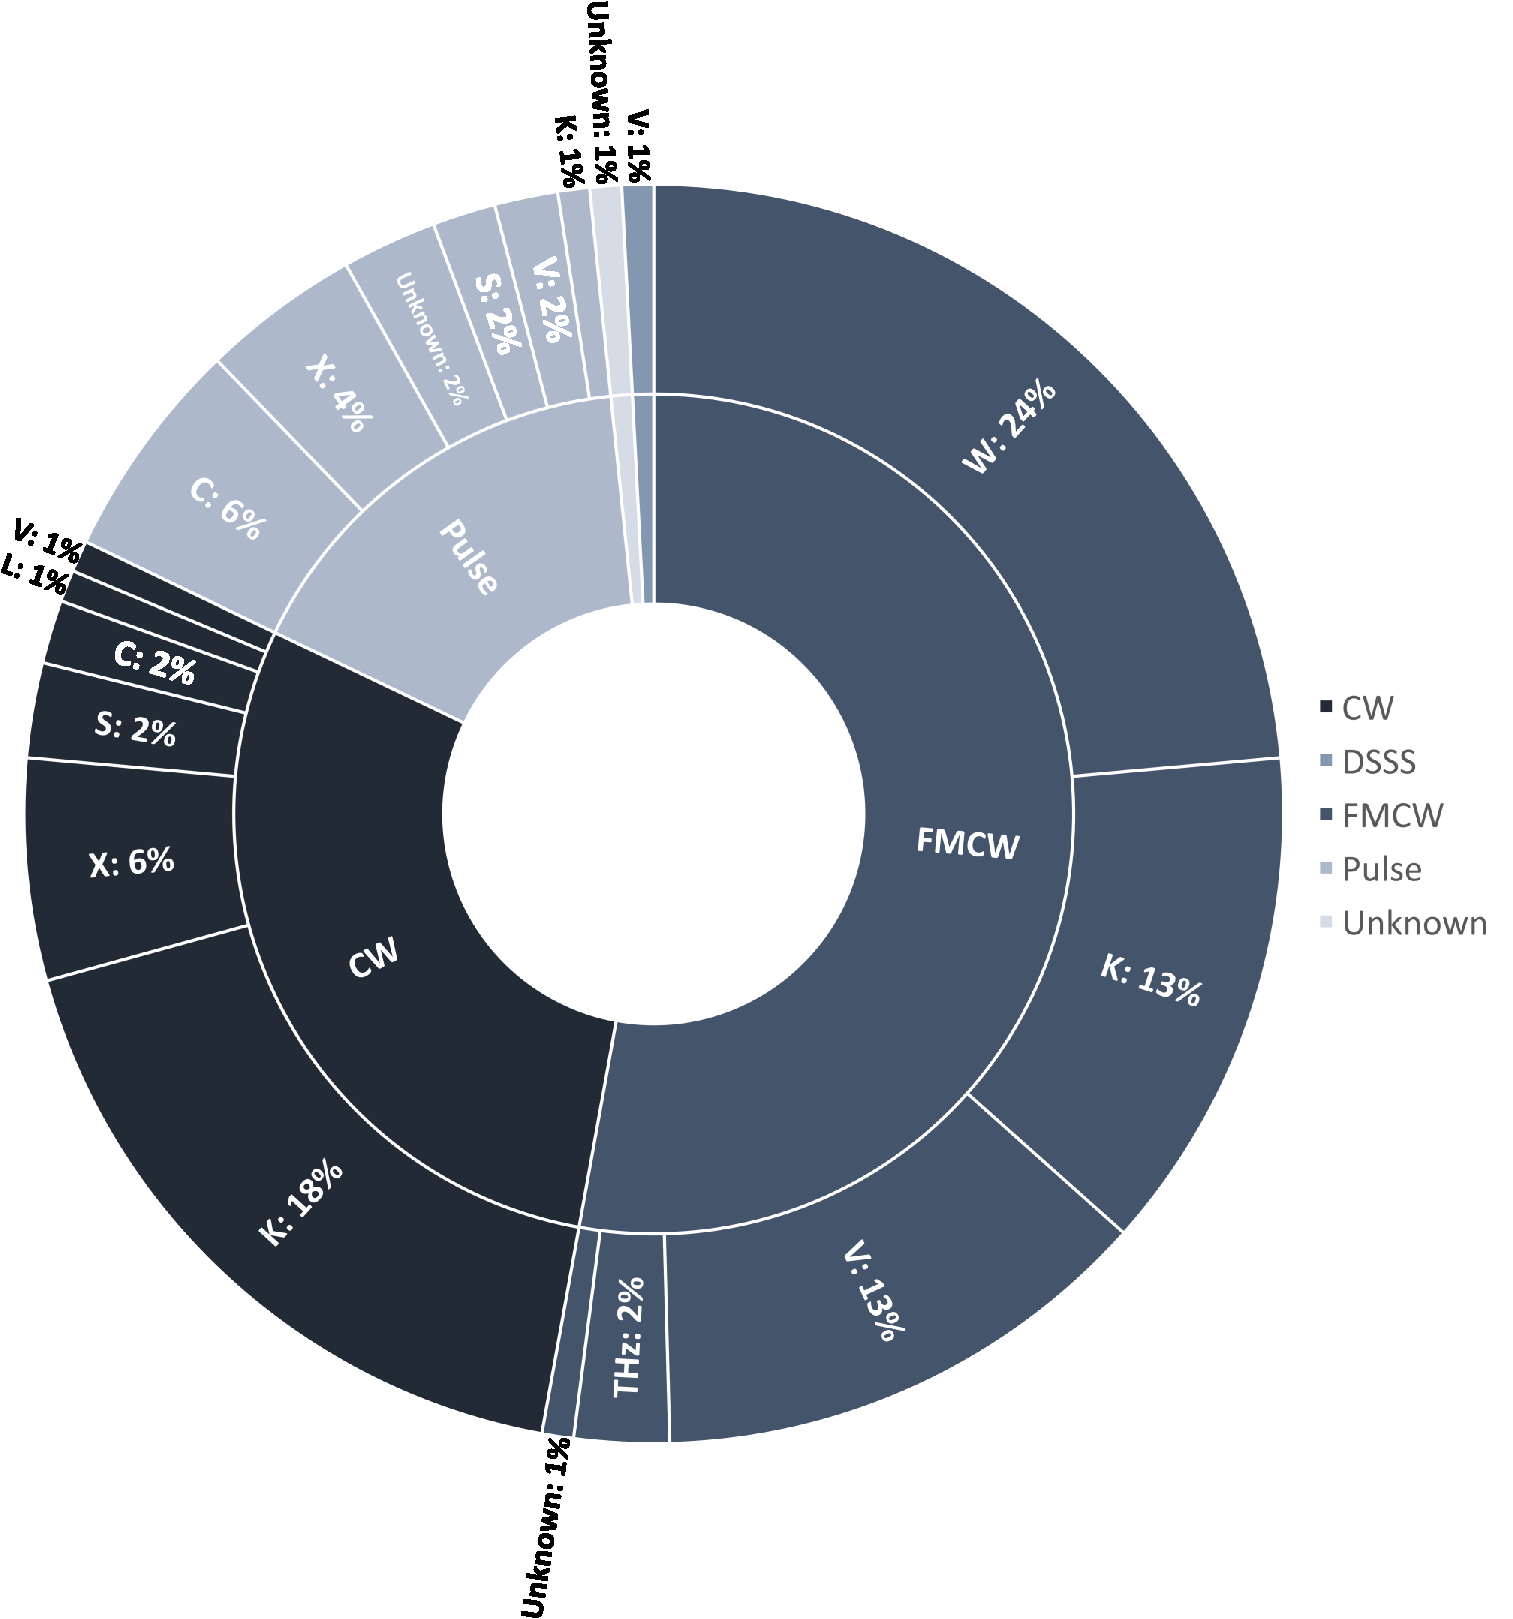
\includegraphics[width=.8\linewidth]{Figures/StateOfTheArt/Radar/diagram-radar-types-frequencies.pdf}
    \vspace{-4pt}
    \caption{Sunburst chart of the radars identified in the SLR. The inner ring and color show the proportion of each radar type, while the outer ring indicates the proportion of each frequency band for each radar type according to the IEEE standard~\cite{IEEE:2020}.}
    \label{fig:state_of_the_art:radar:radars-types-frequencies}
    \vspace{-4pt}
\end{figure}

We also classified radars according to their frequency band according to the IEEE Standard Letter Designations for Radar-Frequency Bands~\cite{IEEE:2020} (\fig~\ref{fig:state_of_the_art:radar:frequencies}). The larger the frequency band, the better resolution the radar provides, and, in principle, the finer the gestures can be acquired. \fig~\ref{fig:state_of_the_art:radar:frequencies} shows that most of the radars ($\frac{88}{123} = 72\%$) operate in the K (18 to 27 GHz, 32\%), V (40 to 75 GHz, 16\%), and W (75 to 110 GHz, 24\%) bands. The V-band encompasses the Google Soli~\cite{Lien:2016}, which operates at 60 GHz and was used in five papers~\cite{Lien:2016,Wang:2016,Copic:2019,Berenguer:2019,Choi:2019} identified by our SLR. Three papers used very high-frequency THz-band radars (300 to 1000 GHz) to achieve better resolution~\cite{Wang:2019b,Wang:2020b,Zhou:2018a}. Only $\frac{27}{123}=22\%$ of the radars operated at frequencies below 18 GHz:
10\% in the X-band (8 to 12 GHz),
7\% in the C-band (4 to 8 GHz),
4\% in the S-band (2 to 4 GHz),
and 1\% in the L-band (1 to 2 GHz). The benefit of lower frequencies is the larger detection range. For a given application, a trade-off has therefore to be chosen between resolution and range. The detection range can also be increased by increasing the transmitted power, but this increases energy consumption and can lead to adverse health effects. 
\fig~\ref{fig:state_of_the_art:radar:radars-types-frequencies} summarizes the distribution of frequency bands by radar type.

Finally, we extracted the radar models used in the papers that provided this information; see \fig~\ref{fig:state_of_the_art:radar:radars}. % shows a wide variety of radar models with a tree map visualization~\cite{Shneiderman:1992}. 
More than a third of the papers ($\frac{46}{123} = 37\%$) did not provide enough information to identify the exact models. Of the 77 remaining publications, we identified 29 unique models %, which depict a rather fragmented landscape. 
with the most popular being the Texas Instruments AWR1642 ($\frac{13}{123} = 11\%$) and IWR1443 ($\frac{5}{123} = 4\%$), the Novelda XeThru X4 ($\frac{9}{123} = 7\%$), the RFBeam K-LC2 ($\frac{8}{123} = 7\%$), and Google Soli ($\frac{6}{123} = 5\%$), respectively. Except for Google Soli, which was designed for integration into smartphones and smart speakers, most of the radar systems from the SLR were not meant for everyday use. However, some of the papers introduce prototypes of radars that could be integrated into furniture~\cite{Mcintosh:2017} or even stitched into clothing~\cite{Wu:2020}.

\begin{figure}[t]
    \centering
    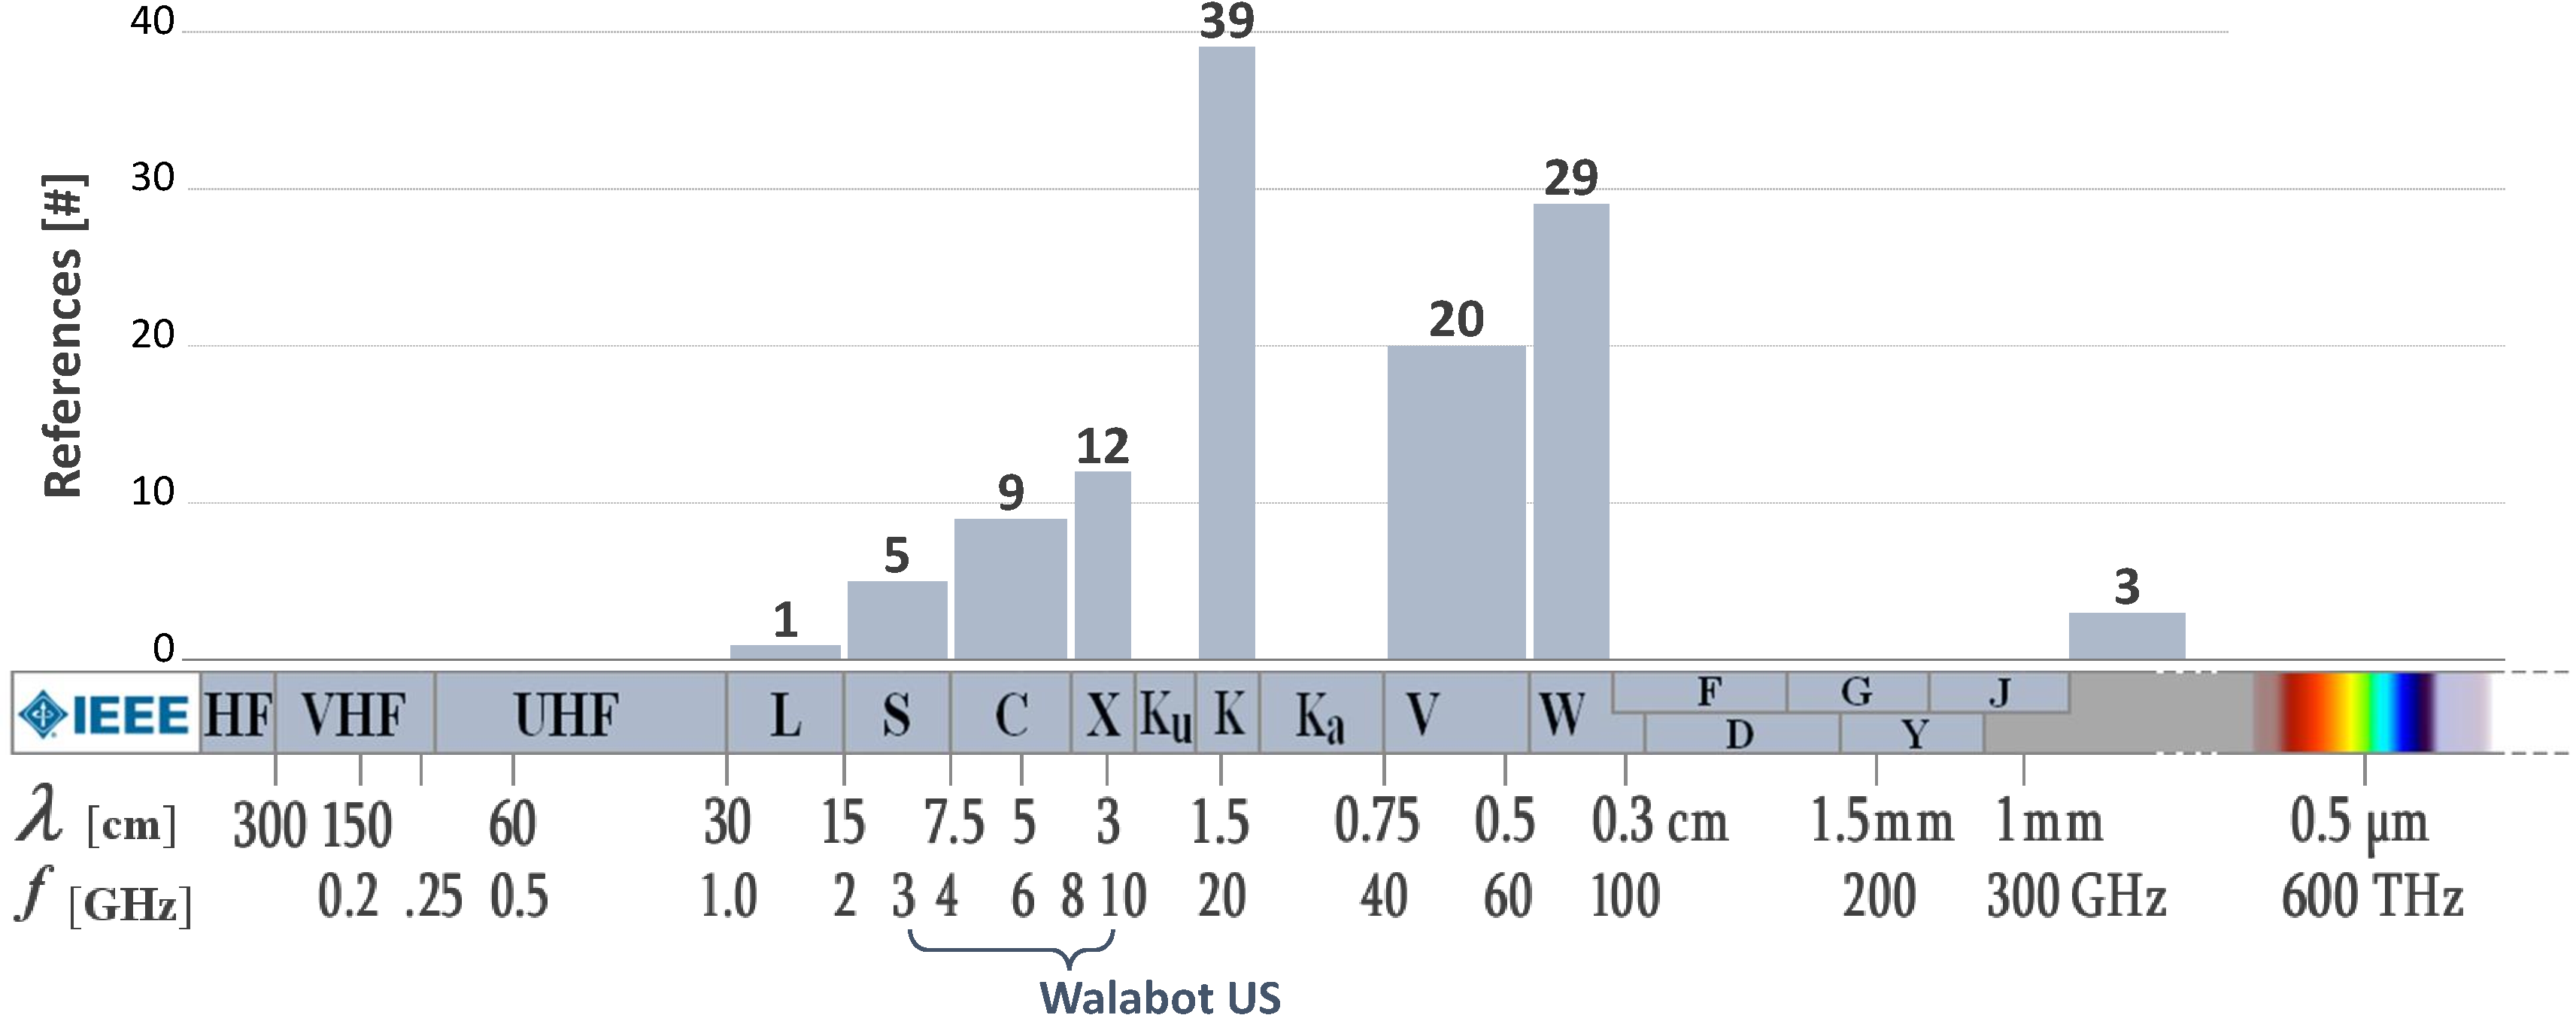
\includegraphics[width=\textwidth]{Figures/StateOfTheArt/Radar/IEEE-bands.pdf}
    \vspace{-12pt}
    \caption{Number of radar systems according to their frequency band~\cite{IEEE:2020} distributed along the electromagnetic continuum (Bottom image of waves and frequency ranges used by radar used with permission from Christian Wolff~\cite{Wolff:2022}), from a total of 118 radars. Five radars did not mention their frequency band.}
    \label{fig:state_of_the_art:IEEE}
    % \vspace{10pt}
\end{figure}

From the above analysis, we make the following observations:
\begin{enumerate}
\setcounter{enumi}{5}
    \item \textit{Predominance of FMCW over other types of radar (\fig~\ref{fig:state_of_the_art:radar:types} and~\ref{fig:state_of_the_art:radar:radars-types-frequencies})}: these radars are the most frequently exploited due to their ability to sense both static and dynamic gestures but also because several models are commercially available. The frequency bands covered by these two categories are high enough to acquire raw data with high resolution.
    \item \textit{Limited coverage of very low/high-frequency bands} (\fig~\ref{fig:state_of_the_art:IEEE}): lower frequencies result in worse range resolution, making it more difficult for the radar to distinguish between two targets. Such radars are thus less interesting for smaller-scale gestures, such as hand and finger gestures, which explains the lower number of works covering these systems. On the contrary, higher frequencies enable better range resolution and thus are better suited for small-scale hand and finger gestures (\eg Google Soli~\cite{Lien:2016,Wang:2016}), at the cost of higher complexity and lower range as the frequency increases. Most systems operate at frequencies between 4 GHz and 100 GHz, which can provide sufficient range resolution with relatively low complexity and power consumption. In addition, some off-the-shelf radar systems used in HCI research were originally developed for other applications and operate specific frequencies, such as collision avoidance systems in cars, which often operate in the K-band. 
\end{enumerate}


%--------------------------------------------------------------------------------%
\subsection{Summary} \label{sec:state_of_the_art:radar:summary}
Radar-based gesture recognition is still in its infancy. Current research mostly focuses on radar systems, signal processing, and algorithms for gesture recognition. As a result, few papers demonstrate a potential use case of their system with a prototype application.
%
In addition, most of the papers rely on deep learning techniques tailored to a specific radar system and gesture set. The combination of a wide variety of sensors, often custom-designed, and a lack of publicly available datasets makes it difficult to reproduce and compare results.

%================================================================================%
\section{Positioning this Work in the Literature} \label{sec:state_of_the_art:this_work}
This chapter provided an overview of gesture-based interaction in the literature. We looked at how to involve users in the development process of gesture-based applications through GESs and identified the main challenges faced by developers when implementing real-time gesture recognition. These challenges include taking into account sensor limitations, extracting gestures from a continuous flow of data, and supporting some variability in the gestures produced by end users.
%
We then had an in-depth look at the LMC, an affordable off-the-shelf device for vision-based gesture recognition. Despite the popularity of this device, most of the papers identified implemented gesture recognition in an opportunistic manner, which could not be adapted easily to support other devices, gestures, or applications. This highlights a need for a tool that would enable the efficient reuse of components designed by, \eg the scientific community, in the development of gesture-based applications.
%
We made several observations regarding three of the four software quality properties defined in Section~\ref{sec:introduction:research:research-questions}.
%
Regarding \textit{maintainability}, we observed a reliance of many papers on non-reusable, often opportunistic, approaches to gesture recognition. As such, supporting other gestures may be impossible without completely re-writing the gesture recognition logic. In addition, we noticed a lack of clear separation of concerns between user interfaces and their gesture recognition logic, which often unnecessarily complicates future modifications.
%
Similarly, the reliance on these opportunistic approaches hinders software \textit{portability}, as they are often tied to the exact sensor used. Supporting other sensors would thus require substantial work. 
%
As for \textit{usability}, the scarcity of tools available to developers presents significant entry barriers for creating highly usable gesture-based applications. Indeed, developing such applications currently requires expertise in gesture recognition, UX design, and application development.

We also looked at radar-based gesture recognition, to identify any application, algorithm, sensor, and dataset described in the literature. 
%
Regarding the \textit{compatibility} software quality property, we observed a scarcity of publicly available datasets and noted that most gesture recognition techniques were tailored for one radar system in particular, making it difficult to reuse datasets across different systems.
%
From a \textit{maintainability} point of view, a majority of the analyzed papers relied on deep learning techniques for gesture recognition. While effective, they posed a challenge for future updates, as changing the sensor or the gesture set could require extensive re-training to achieve the same level of performance.
%
In terms of \textit{portability}, we did not observe any consensus on an affordable and efficient off-the-shelf radar sensor, resulting in a plethora of different (custom) radar systems. Making matters worse, a large part of the proposed gesture recognition techniques were specific to one sensor and gesture set, which limited their applicability to other applications.
%
Regarding \textit{usability}, we noticed that very few papers demonstrated potential use cases of their system with prototype applications. In addition, most of the proposed techniques could not support user-submitted gestures without extensive re-training, which could negatively impact usability, should they be used in real applications~\cite{Nacenta:2013}.

In conclusion, most of the papers that we analyzed in this chapter did not properly address four of the ISO/IEC 25010 software quality properties~\cite{iso25010}, namely compatibility, maintainability, portability, and usability. 
%
Having identified the main challenges of (radar-based) gesture recognition, the rest of this thesis will focus on the development of tools and methods that streamline the development of highly usable gesture interfaces.
